\documentclass[12pt]{article}
\usepackage{lmodern}
\usepackage{amssymb,amsmath}
\usepackage{ifxetex,ifluatex}
\usepackage{fixltx2e} % provides \textsubscript
\ifnum 0\ifxetex 1\fi\ifluatex 1\fi=0 % if pdftex
  \usepackage[T1]{fontenc}
  \usepackage[utf8]{inputenc}
\else % if luatex or xelatex
  \ifxetex
    \usepackage{mathspec}
  \else
    \usepackage{fontspec}
  \fi
  \defaultfontfeatures{Ligatures=TeX,Scale=MatchLowercase}
\fi
% use upquote if available, for straight quotes in verbatim environments
\IfFileExists{upquote.sty}{\usepackage{upquote}}{}
% use microtype if available
\IfFileExists{microtype.sty}{%
\usepackage{microtype}
\UseMicrotypeSet[protrusion]{basicmath} % disable protrusion for tt fonts
}{}
\usepackage[left=2.5cm,right=2.5cm,top=2.5cm,bottom=2.5cm,headheight=12pt,letterpaper]{geometry}
\usepackage{hyperref}
\hypersetup{unicode=true,
            pdftitle={Hierarchical Generalized Additive Models in ecology: an introduction with mgcv},
            pdfborder={0 0 0},
            breaklinks=true}
\urlstyle{same}  % don't use monospace font for urls
\usepackage{color}
\usepackage{fancyvrb}
\newcommand{\VerbBar}{|}
\newcommand{\VERB}{\Verb[commandchars=\\\{\}]}
\DefineVerbatimEnvironment{Highlighting}{Verbatim}{commandchars=\\\{\}}
% Add ',fontsize=\small' for more characters per line
\usepackage{framed}
\definecolor{shadecolor}{RGB}{248,248,248}
\newenvironment{Shaded}{\begin{snugshade}}{\end{snugshade}}
\newcommand{\KeywordTok}[1]{\textcolor[rgb]{0.13,0.29,0.53}{\textbf{#1}}}
\newcommand{\DataTypeTok}[1]{\textcolor[rgb]{0.13,0.29,0.53}{#1}}
\newcommand{\DecValTok}[1]{\textcolor[rgb]{0.00,0.00,0.81}{#1}}
\newcommand{\BaseNTok}[1]{\textcolor[rgb]{0.00,0.00,0.81}{#1}}
\newcommand{\FloatTok}[1]{\textcolor[rgb]{0.00,0.00,0.81}{#1}}
\newcommand{\ConstantTok}[1]{\textcolor[rgb]{0.00,0.00,0.00}{#1}}
\newcommand{\CharTok}[1]{\textcolor[rgb]{0.31,0.60,0.02}{#1}}
\newcommand{\SpecialCharTok}[1]{\textcolor[rgb]{0.00,0.00,0.00}{#1}}
\newcommand{\StringTok}[1]{\textcolor[rgb]{0.31,0.60,0.02}{#1}}
\newcommand{\VerbatimStringTok}[1]{\textcolor[rgb]{0.31,0.60,0.02}{#1}}
\newcommand{\SpecialStringTok}[1]{\textcolor[rgb]{0.31,0.60,0.02}{#1}}
\newcommand{\ImportTok}[1]{#1}
\newcommand{\CommentTok}[1]{\textcolor[rgb]{0.56,0.35,0.01}{\textit{#1}}}
\newcommand{\DocumentationTok}[1]{\textcolor[rgb]{0.56,0.35,0.01}{\textbf{\textit{#1}}}}
\newcommand{\AnnotationTok}[1]{\textcolor[rgb]{0.56,0.35,0.01}{\textbf{\textit{#1}}}}
\newcommand{\CommentVarTok}[1]{\textcolor[rgb]{0.56,0.35,0.01}{\textbf{\textit{#1}}}}
\newcommand{\OtherTok}[1]{\textcolor[rgb]{0.56,0.35,0.01}{#1}}
\newcommand{\FunctionTok}[1]{\textcolor[rgb]{0.00,0.00,0.00}{#1}}
\newcommand{\VariableTok}[1]{\textcolor[rgb]{0.00,0.00,0.00}{#1}}
\newcommand{\ControlFlowTok}[1]{\textcolor[rgb]{0.13,0.29,0.53}{\textbf{#1}}}
\newcommand{\OperatorTok}[1]{\textcolor[rgb]{0.81,0.36,0.00}{\textbf{#1}}}
\newcommand{\BuiltInTok}[1]{#1}
\newcommand{\ExtensionTok}[1]{#1}
\newcommand{\PreprocessorTok}[1]{\textcolor[rgb]{0.56,0.35,0.01}{\textit{#1}}}
\newcommand{\AttributeTok}[1]{\textcolor[rgb]{0.77,0.63,0.00}{#1}}
\newcommand{\RegionMarkerTok}[1]{#1}
\newcommand{\InformationTok}[1]{\textcolor[rgb]{0.56,0.35,0.01}{\textbf{\textit{#1}}}}
\newcommand{\WarningTok}[1]{\textcolor[rgb]{0.56,0.35,0.01}{\textbf{\textit{#1}}}}
\newcommand{\AlertTok}[1]{\textcolor[rgb]{0.94,0.16,0.16}{#1}}
\newcommand{\ErrorTok}[1]{\textcolor[rgb]{0.64,0.00,0.00}{\textbf{#1}}}
\newcommand{\NormalTok}[1]{#1}
\usepackage{graphicx,grffile}
\makeatletter
\def\maxwidth{\ifdim\Gin@nat@width>\linewidth\linewidth\else\Gin@nat@width\fi}
\def\maxheight{\ifdim\Gin@nat@height>\textheight\textheight\else\Gin@nat@height\fi}
\makeatother
% Scale images if necessary, so that they will not overflow the page
% margins by default, and it is still possible to overwrite the defaults
% using explicit options in \includegraphics[width, height, ...]{}
\setkeys{Gin}{width=\maxwidth,height=\maxheight,keepaspectratio}
\IfFileExists{parskip.sty}{%
\usepackage{parskip}
}{% else
\setlength{\parindent}{0pt}
\setlength{\parskip}{6pt plus 2pt minus 1pt}
}
\setlength{\emergencystretch}{3em}  % prevent overfull lines
\providecommand{\tightlist}{%
  \setlength{\itemsep}{0pt}\setlength{\parskip}{0pt}}
\setcounter{secnumdepth}{0}
% Redefines (sub)paragraphs to behave more like sections
\ifx\paragraph\undefined\else
\let\oldparagraph\paragraph
\renewcommand{\paragraph}[1]{\oldparagraph{#1}\mbox{}}
\fi
\ifx\subparagraph\undefined\else
\let\oldsubparagraph\subparagraph
\renewcommand{\subparagraph}[1]{\oldsubparagraph{#1}\mbox{}}
\fi

%%% Use protect on footnotes to avoid problems with footnotes in titles
\let\rmarkdownfootnote\footnote%
\def\footnote{\protect\rmarkdownfootnote}


  \title{Hierarchical Generalized Additive Models in ecology: an introduction
with mgcv}
    \author{}
    \date{}
  
\usepackage{booktabs}
\usepackage{longtable}
\usepackage{array}
\usepackage{multirow}
\usepackage{wrapfig}
\usepackage{float}
\usepackage{colortbl}
\usepackage{pdflscape}
\usepackage{tabu}
\usepackage{threeparttable}
\usepackage{threeparttablex}
\usepackage[normalem]{ulem}
\usepackage{makecell}
\usepackage{lineno}
\usepackage{placeins}
\usepackage{authblk}

\linenumbers

\author[1,2,*]{Eric J. Pedersen}
\author[3,4]{David L. Miller}
\author[5]{Gavin L. Simpson}
\author[6]{Noam Ross}
\affil[1]{Northwest Atlantic Fisheries Center, Fisheries and Oceans Canada, St. John's, NL, Canada}
\affil[2]{Department of Biology, Memorial University, St. John's, NL, Canada}
\affil[3]{Centre for Research into Ecological and Environmental Modelling, University of St Andrews, St Andrews, UK}
\affil[4]{School of Mathematics and Statistics, University of St Andrews, St Andrews, UK}
\affil[5]{Institute of Environmental Change and Society, University of Regina, Regina, SK, Canada}
\affil[6]{Ecohealth Alliance, New York, NY, USA}
\affil[*]{Corresponding author. Email: eric.j.pedersen@gmail.com}

\begin{document}
\maketitle

\section{Abstract}\label{abstract}

In this paper, we discuss an extension to two popular approaches to
modelling complex structures in ecological data: the generalized
additive model (GAM) and the hierarchical model (HGLM). The hierarchical
GAM (HGAM), allows modelling of nonlinear functional relationships
between covariates and outcomes where the shape of the function itself
varies between different grouping levels. We describe the theoretical
connection between these models, HGLMs and GAMs, explain how to model
different assumptions about the degree of inter-group variability in
functional response, and show how HGAMs can be readily fitted using
existing GAM software, the mgcv package in R. We also discuss
computational and statistical issues with fitting these models, and
demonstrate how to fit HGAMs on example data.

\section{I: Introduction}\label{i-introduction}

Two of the most popular and powerful modelling techniques currently in
use by ecologists are generalized additive models (GAMs; Wood, 2017a)
for modelling flexible regression functions, and generalized linear
mixed models (``hierarchical generalized linear models'' (HGLMs) or
simply ``hierarchical models''; Bolker et al., 2009; Gelman et al.,
2013) for modelling between-group variability in regression
relationships.

At first glance, GAMs and HGLMs are very different tools used to solve
different problems. GAMs are used to estimate smooth functional
relationships between predictor variables and the response. HGLMs, on
the other hand, are used to estimate linear relationships between
predictor variables and response (although nonlinear relationships can
also be modeled through quadratic terms or other transformations of the
predictor variables), but impose a structure where predictors are
organized into groups (often referred to as ``blocks'') and the
relationships between predictor and response may vary across groups.
Either the slope or intercept, or both, may be subject to grouping. A
typical example of HGLM use might be to include site-specific effects in
a model of population counts, or to model individual level heterogeneity
in a study with repeated observations of multiple individuals.

However, the connection between HGLMs and GAMs is quite deep, both
conceptually and mathematically (Verbyla et al., 1999). HGLMs and GAMs
fit highly variable models by ``pooling'' parameter estimates towards
one another, by penalizing squared deviations from some simplier model.
In an HGLM, this occurs as group-level effects are pulled towards global
effects (penalizing the squared differences between each group-level
parameter estimate and the global effect). In a GAM, this occurs in the
enforcement of a smoothness criterion on the variability of a functional
relationship, pulling parameters towards some function that is assumed
to be totally smooth (such as a straight line) by penalizing squared
deviations from that totally smooth function.

Given this connection, a natural extension to the standard GAM framework
is to allow smooth functional relationships between predictor and
response to vary between groups, but in such a way that the different
functions are in some sense pooled toward a common shape. We often want
to know both how functional relationships vary between groups, and if a
relationship holds across groups. We will refer to this type of model as
a \emph{hierarchical GAM}, or HGAM.

There are many potential uses for HGAMs. For example, we can use HGAMs
to estimate how the maximum size of different fish species varies along
a common temperature gradient (figure \ref{fig:fish_size}). Each species
will typically have its own response function, but since the species
overlap in range, they should have similar responses over at least some
of the temperature gradient; figure \ref{fig:fish_size} shows all three
species reach their largest maximum sizes in the centre of the
temperature gradient. Estimating a separate function for each species
throws away a lot of shared information and could result in highly noisy
function estimates if there were only a few data points for each
species. Estimating a single average relationship could result in a
function that did not predict any specific group well. In our example,
using a single global temperature-size relationship would miss that the
three species have distinct temperature optima, and that the orange
species is significantly smaller at all temperatures than the other two
(figure \ref{fig:fish_size}). We prefer a hierarchical model that
includes a global temperature-size curve plus species-specific curves
that were penalized to be close to the mean function.

\begin{figure}

{\centering 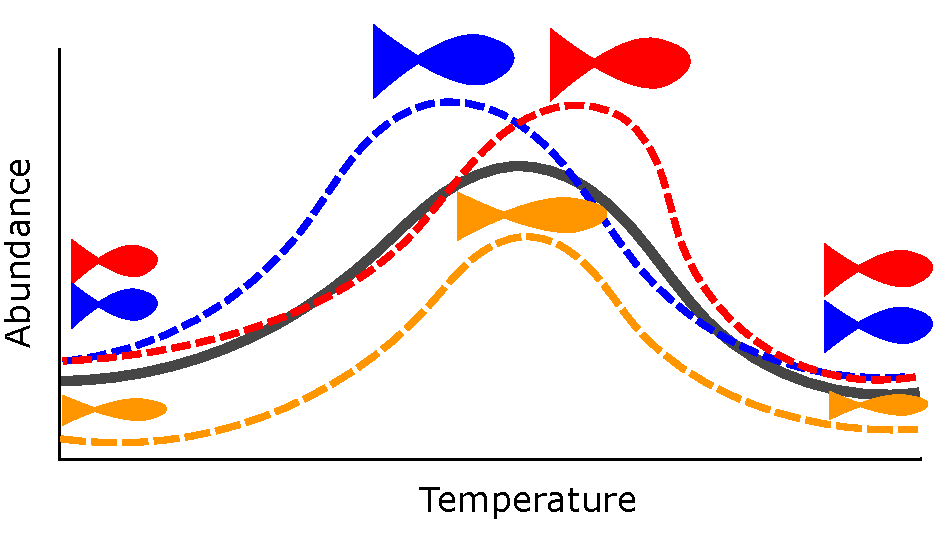
\includegraphics[width=.6\linewidth]{../figures/temp_growth_example} 

}

\caption{\label{fig:fish_size}Hypothetical example of functional variability between different group levels. Each line indicates how the abundance for different species of fish in a community might vary as a function of average water temperature. The orange species shows lower abundance at all temperatures, and the red and blue species differ at which temperature they can achieve the maximum possible size. However, all three curves are similiarly smooth and peak close to one another relative to the entire range of tested temperatures.}\label{fig:fish_size}
\end{figure}

This paper discusses several approaches to group-level smoothing, and
corresponding trade-offs. We focus on fitting HGAMs with the popular
\textbf{mgcv} package for the R statistical programming language, which
allows for a variety of HGAM model structures and fitting strategies. We
discuss options available to the modeller and practical and theoretical
reasons for choosing them. We demonstrate the different approaches
across a range of case studies.

This paper is divided into five sections. Part II is a brief review of
how GAMs work and their relation to hierarchical models. In part III, we
discuss different HGAM formulations, what assumptions each model makes
about how information is shared between groups, and different ways of
specifying these models in \textbf{mgcv}. In part IV, we work through
example analyses using this approach, to demonstrate the modelling
process and how HGAMs can be incorporated into the ecologist's
quantitative toolbox. Finally, in part V, we discuss some of the
computational and statistical issues involved in fitting HGAMs in
\textbf{mgcv}. We have also included all the code needed to reproduce
the results in this manuscript in supplemental code (online), and on the
GitHub repository associated with this paper
\href{http://www.github.com/noamross/mixed-effect-gams}{github.com/noamross/mixed-effect-gams}.

\FloatBarrier

\section{II: A review of Generalized Additive
Models}\label{ii-a-review-of-generalized-additive-models}

The generalized linear model (GLM; McCullagh \& Nelder, 1989) relates
the mean of a response (\(y\)) to a linear combination of explanatory
variables. The response is assumed to be conditionally distributed
according to some exponential family distribution (e.g., binomial,
Poisson or Gamma distributions for trial, count or strictly positive
real response, respectively). The generalized additive model (GAM;
Hastie \& Tibshirani, 1990; Ruppert, Wand \& Carroll, 2003; Wood, 2017a)
allows the relationships between the explanatory variables (henceforth
covariates) and the response to be described by smooth curves (usually
\emph{splines} (de Boor, 1978), but potentially other structures). In
general we have models of the form: \[
\mathbb{E}\left( Y \right) = g^{-1}\left( \beta_0 + \sum_{j=1}^J f_j(x_j) \right)\,,
\] where \(\mathbb{E}(Y)\) is the expected value of the response \(Y\)
(with an appropriate distribution and link function \(g\)), \(f_j\) is a
smooth function of the covariate \(x_j\), \(\beta_0\) is an intercept
term and \(g^{-1}\) is the inverse link function. Hereafter, we will
refer to these smooth functions as \emph{smoothers}. In the example
equation above, there are \(J\) smoothers and each is a function of only
one covariate, though it is possible to construct smoothers of multiple
variables.

Each smoother \(f_j\) is represented by a sum of \(K\) simpler, fixed
\emph{basis functions} (\(b_{j,k}\)) multiplied by corresponding
coefficients (\(\beta_{j,k}\)), which need to be estimated: \[
f_j(x_j) = \sum_{k=1}^K \beta_{j,k} b_{j,k}(x_j).
\] \(K\), referred to as ``basis size'', ``basis complexity'' or ``basis
richness'', determines the maximum complexity of each smoother.

It would seem that large basis size could lead to overfitting, but this
counteracted by a \emph{smoothing penalty} that influences basis
function coefficients so as to prevent excess wiggliness and ensure that
appropriate complexity of each smoother. For each smoother, one or more
\emph{penalty matrices} \((\mathbf{S})\), specific to the form of the
basis functions, is pre- and post-multiplied by the parameter vector
\(\boldsymbol{\beta}\) to calculate the penalty
\((\boldsymbol{\beta}^T \mathbf{S} \boldsymbol{\beta})\). A penalty term
is then added to the model log-likelihood \(L\), controlling the
trade-off via a \emph{smoothing parameter} (\(\lambda\)). The penalized
log-likelihood used to fit the model is thus: \[
L - \boldsymbol{\lambda} \boldsymbol{\beta}^T \mathbf{S} \boldsymbol{\beta}
\]

Figure \ref{fig:smoothing_effect} shows an example of how different
choices of the smoothing parameter (\(\lambda\)) affect the shape of the
resulting smoother. Data (points) were generated from the blue function
and noise added to them. In the left plot \(\lambda\) was selected using
Restricted Maximum Likelihood (REML) to give a good fit to the data, in
the middle plot \(\lambda\) was set to zero, so the penalty has no
effect and the function interpolates the data, the right plot shows when
\(\lambda\) is set to a very large value, so the penalty removes all
terms that have any wiggliness, giving a straight line.

To measure the complexity of a penalized smooth terms we use the
\emph{effective degrees of freedom} (EDF), which at a maximum is the
number of coefficients to be estimated in the model, minus any
constraints. The EDF can take non-integer values and larger values
indicate more wiggly terms (see Wood (2017a, Section 6.1.2) for further
details). The number of basis functions, \(k\) sets a maximum for the
EDF, as a smoother cannot have more than \(k\) EDF. When the EDF is well
below \(k\), increasing \(k\) generally has very little effect on the
shape of the function. In general, \(k\) should be set large enough to
allow for potential variation in the smoother while still staying low
enough to keep computation time low (see section V for more on this). In
\textbf{mgcv}, the function \texttt{mgcv::check.gam} can be used to
determine if \(k\) has been set too low.

\begin{figure}
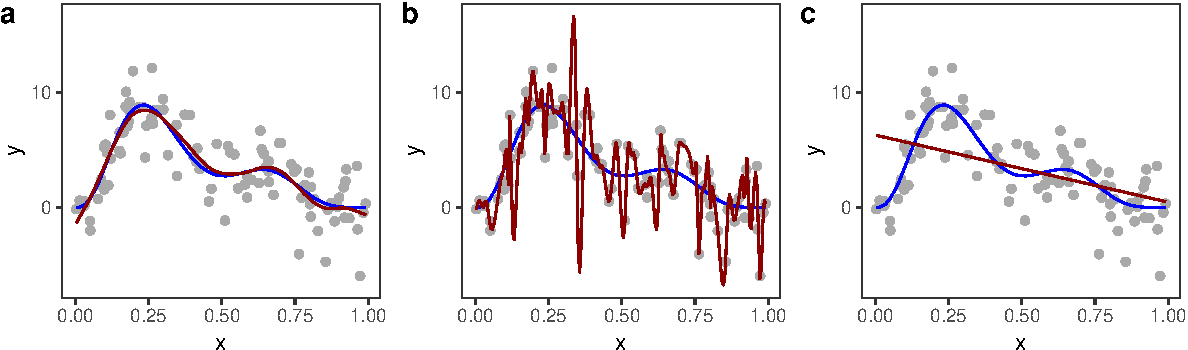
\includegraphics[width=\linewidth]{../figures/lambda-1} \caption{\label{fig:smoothing_effect}Effect of different choices of smoothing parameter ($\lambda$) on the shape of the resulting smoother. Left:  $\lambda$ estimated using REML; middle: $\lambda$ set to zero (no smoothing); Right: $\lambda$ is set to a very large value.}\label{fig:lambda}
\end{figure}

Random effects are also ``smooths'' in this framework. In this case, the
penalty matrix is the inverse of the correlation matrix of the basis
function coefficients (Kimeldorf \& Wahba, 1970; Wood, 2017a). To
include a simple single-level random effect to account for variation in
group means (intercepts) there will be one basis function for each level
of the grouping variable, that takes a value of 1 for any observation in
that group and 0 for any observation not in the group. The penalty
matrix for these terms is a \(n_g\) by \(n_g\) identity matrix, where
\(n_g\) is the number of groups. This means that each group-level
coefficient will be penalized in proportion to its squared deviation
from zero. This is equivalent to how random effects are estimated in
standard mixed effect models. The penalty term is then proportional to
the inverse of the variance of the fixed effect estimated by standard
hierarchical model software (Verbyla et al., 1999).

This connection between random effects and splines extends beyond the
varying-intercept case. Any single-penalty basis-function representation
of a smooth can be transformed so that it can be represented as a
combination of a random effect with an associated variance, and possibly
one or more fixed effects. See Verbyla et al. (1999) or Wood, Scheipl \&
Faraway (2013) for a more detailed discussion on the connections between
these approaches.

\subsubsection{Basis types and penalty
matrices}\label{basis-types-and-penalty-matrices}

Different types of smoothers are useful for different needs, and have
different associated penalty matrices for their basis function
coefficients. In the examples in this paper, we will use three types of
smoothers: thin plate regression splines, cyclic cubic smoothers, and
random effects.

Thin plate regression splines (TPRS; Wood, 2003), are a general purpose
spline basis which can be used for problems in any number of dimensions,
provided one can assume that the amount of smoothing in any of the
covariates is the same (so called isotropy or rotational invariance).
TPRS, like many splines, use a penalty matrix made up of terms based on
the the integral of the squared derivatives of basis functions across
their range (see Wood (2017a) page 216 for details on this penalty).
Models that overfit the data will tend to have large derivatives, so
this penalization reduces wiggliness. We will refer to the order of
penalized derivatives as \(m\). Typically, TPRS are second-order
(\(m=2\)), meaning that the penalty is proportionate to the integral of
the squared second derivative. However, TPRS may be of lower order
(\(m=1\), penalizing squared first derivatives), or higher order
(\(m > 2\), penalizing squared higher order derivatives). We will see in
section III how lower-order TPRS smoothers are useful in fitting HGAMs.
Example basis functions and penalty matrix \(\mathbf{S}\) for a \(m=2\)
TPRS with six basis functions for evenly spaced data are shown in figure
\ref{fig:basis_example}.

Cyclic cubic smoothers are another smoother that penalizes the squared
second derivative of the smooth across the function. In these, though,
start and end of the smoother are constrained to match in value and
first derivative. These are useful for fitting models with cyclic
components such as seasonal effects. We will use these smoothers to
demonstrate how to fit HGAMs to cyclic data.

\subsubsection{Smoothing penalties vs.~shrinkage
penalties}\label{smoothing-penalties-vs.shrinkage-penalties}

Penalties can have two effects on how well a model fits: they can
penalize how wiggly a given term is (smoothing) and they can penalize
the absolute size of the function (shrinkage). The penalty can only
affect the components of the smoother that have derivatives (the
\emph{range space}), not the other parts (the \emph{null space}). For
1-dimensional thin plate regression splines (when \(m=2\)), this means
that there is a linear term left in the model, even when the penalty is
in full force (as \(\lambda \rightarrow \infty\)), as shown in figure
\ref{fig:basis_example} (this is also why
figure~\ref{fig:smoothing_effect}c resulted in a linear, rather than
flat, fit to the data). The random effects smoother we discussed earlier
is an example of a pure shrinkage penalty; it penalizes all deviations
away from zero, no matter the pattern of those deviations. This will be
useful later in section III, where we use random effect smoothers as one
of the components of a HGAM.

\begin{figure}
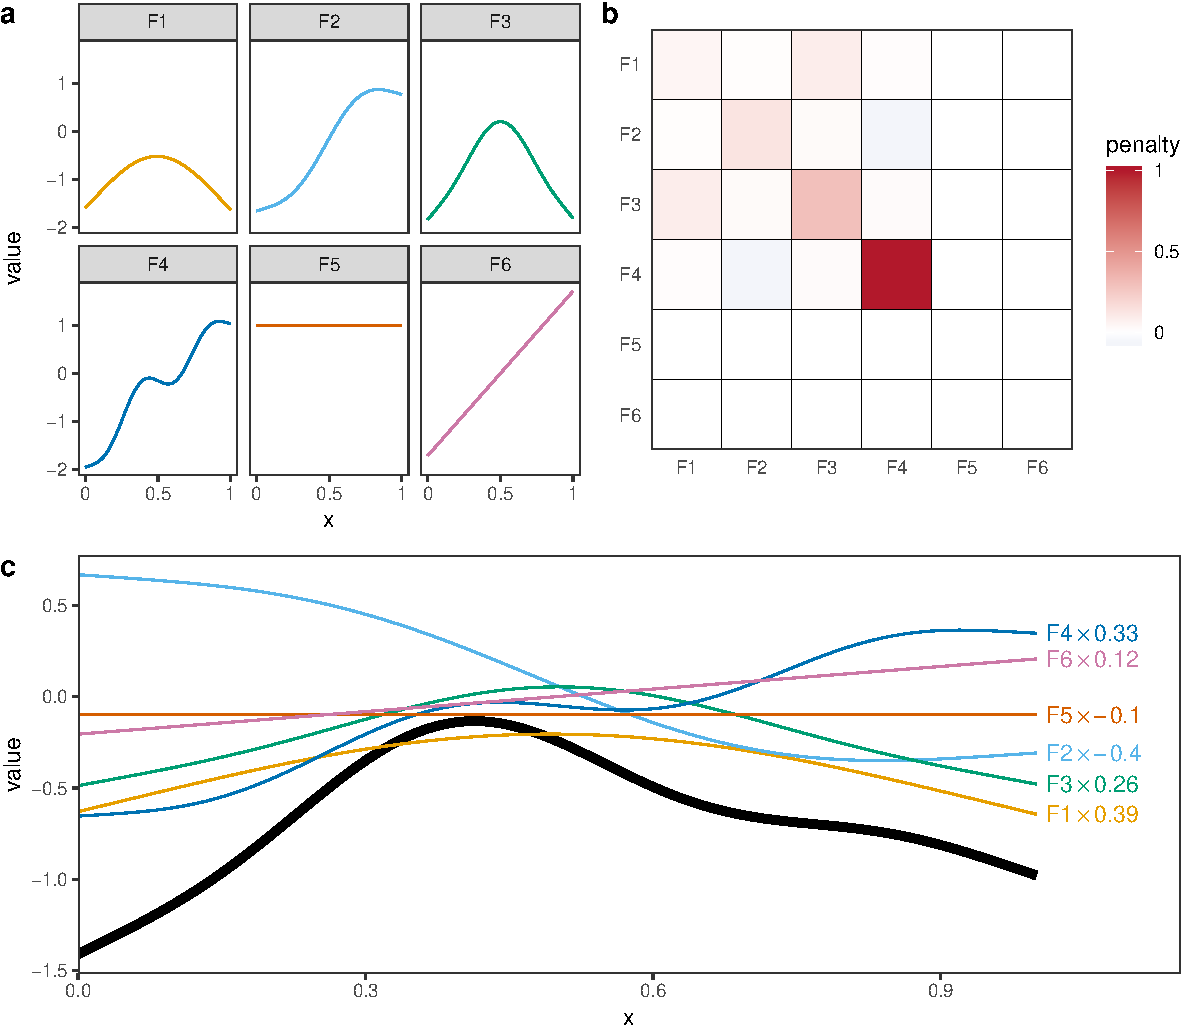
\includegraphics[width=\linewidth]{../figures/basis_function_examples-1} \caption{\label{fig:basis_example}a) Examples of the basis functions associated with a six basis function thin plate spline (m=2), calculated for data, $x$, spread evenly between $x=0$ and $x=1$. Each line represents a single basis function. b) The smoothing  penalty matrix for the thin plate smoother. Red entries indicate positive values and blue indicate negative values.  For example, functions F3 and F4 would have the greatest proportionate effect on the total penalty (as they have the largest values on the diagonal), whereas function F5 and F6 would not contribute to the wiggliness penalty at all (all the values in the 5th and 6th row and column of the penalty matrix are zero). This means these functions are in the null space of the penalty matrix, and are treated as completely smooth. c) An example of how the basis functions add up to create a single smooth function. Thin coloured lines represent each basis function multiplied by a coefficient, and the solid black line is the sum of those basis functions.}\label{fig:basis_function_examples}
\end{figure}

\subsection{Interactions between smooth
terms}\label{interactions-between-smooth-terms}

It is also possible to create interactions between covariates with
different smoothers (or degrees of smoothness) assumed for each
covariate, using \emph{tensor products}. For instance, if one wanted to
estimate the interacting effects of temperature and time (in seconds) on
some outcome, it would not make sense to use a two-dimensional TPRS
smoother, as that would assume that a one degree change in temperature
would equate to a one second change in time. Instead, a tensor product
allows us to create a new set of basis functions that allow for each
marginal function (here temperature and time) to have its own marginal
smoothness penalty. A different basis can be used in each marginal
smooth, as required for the data at hand.

There are two approaches used in \textbf{mgcv} for generating tensor
products. The first approach (Wood, 2006a) essentially creates an
interaction of each pair of basis functions for each marginal term, and
a penalty for each marginal term that penalizes the average wiggliness
in that term; in \textbf{mgcv}, these are created using the
\texttt{te()} function. The second approach (Wood, Scheipl \& Faraway,
2013) separates each penalty into penalized (range space) and
unpenalized components (null space; components that don't have
derivatives, such as intercept and linear terms in a one-dimensional
cubic spline), then creates new basis functions and penalties for all
pair-wise combinations of penalized and unpenalized components between
all pairs of marginal bases; in \textbf{mgcv}, these are created using
the \texttt{t2()} function. The advantage of the first method is that it
requires fewer smoothing parameters, so is faster to estimate in most
cases. The advantage of the second method is that the tensor products
created this way only have a single penalty associated with each
marginal basis (unlike the \texttt{te()} approach, where each penalty
applies to all basis functions), so it can be fitted using standard
mixed effect software such as \textbf{lme4} (Bates et al., 2015).

\subsection{Comparison to hierarchical linear
models}\label{comparison-to-hierarchical-linear-models}

Hierarchical generalized linear models (Gelman, 2006; HGLMs; also
referred to as generalized linear mixed effect models, multilevel models
etc; e.g., Bolker et al., 2009) are an extension of regression modelling
that allows the inclusion of terms in the model that account for
structure in the data --- the structure is usually of the form of a
nesting of the observations. For example, in an empirical study,
individuals may be nested within sample sites, sites are nested within
forests, and forests within provinces. The depth of the nesting is
limited by the fitting procedure and number of parameters to estimate.

HGLMs are a highly flexible way to think about grouping in ecological
data; the groupings used in models often refer to the spatial or
temporal scale of the data (McMahon \& Diez, 2007) though can be based
on any useful grouping.

We would like to be able to think about the groupings in our data in a
similar way, even when the covariates in our model are related to the
response in a smooth way. The next section investigates the extension of
the smoothers we showed above to the case where observations are grouped
and we model group-level smoothers. \FloatBarrier

\section{III: What are hierarchical
GAMs?}\label{iii-what-are-hierarchical-gams}

\subsection{What do we mean by hierarchical
smoothers?}\label{what-do-we-mean-by-hierarchical-smoothers}

In this section, we will describe how to model inter-group variability
using smooth curves and how to fit these models using \textbf{mgcv}.
Model structure is key in this framework, so we start with three model
choices:

\begin{enumerate}
\def\labelenumi{\arabic{enumi}.}
\tightlist
\item
  Should each group have its own smoother, or will a common smoother
  suffice?
\item
  Do all of the group-specific smoothers have the same wiggliness, or
  should each group have its own smoothing parameter?
\item
  Will the smoothers for each group have a similar shape to one another
  --- a shared global smoother?
\end{enumerate}

These three choices result in five possible models (figure
\ref{fig:models}):

\begin{enumerate}
\def\labelenumi{\arabic{enumi}.}
\tightlist
\item
  A single common smoother for all observations; We will refer to this
  as model \emph{G}, as it only has a Global smoother.
\item
  A global smoother plus group-level smoothers that have the same
  wiggliness. We will refer to this as model \emph{GS} (for Global
  smoother with individual effects with a Shared penalty)
\item
  A global smoother plus group-level smoothers with differing
  wiggliness. We will refer to this as model \emph{GI} (for Global
  smoother with individiual effects with Individual penalties)
\item
  Group-specific smoothers without a global smoother, but with all
  smoothers having the same wiggliness. We will refer to this as model
  \emph{S}.
\item
  Group-specific smoothers with different wiggliness. We will refer to
  this as model \emph{I}.
\end{enumerate}

\begin{figure}
\centering
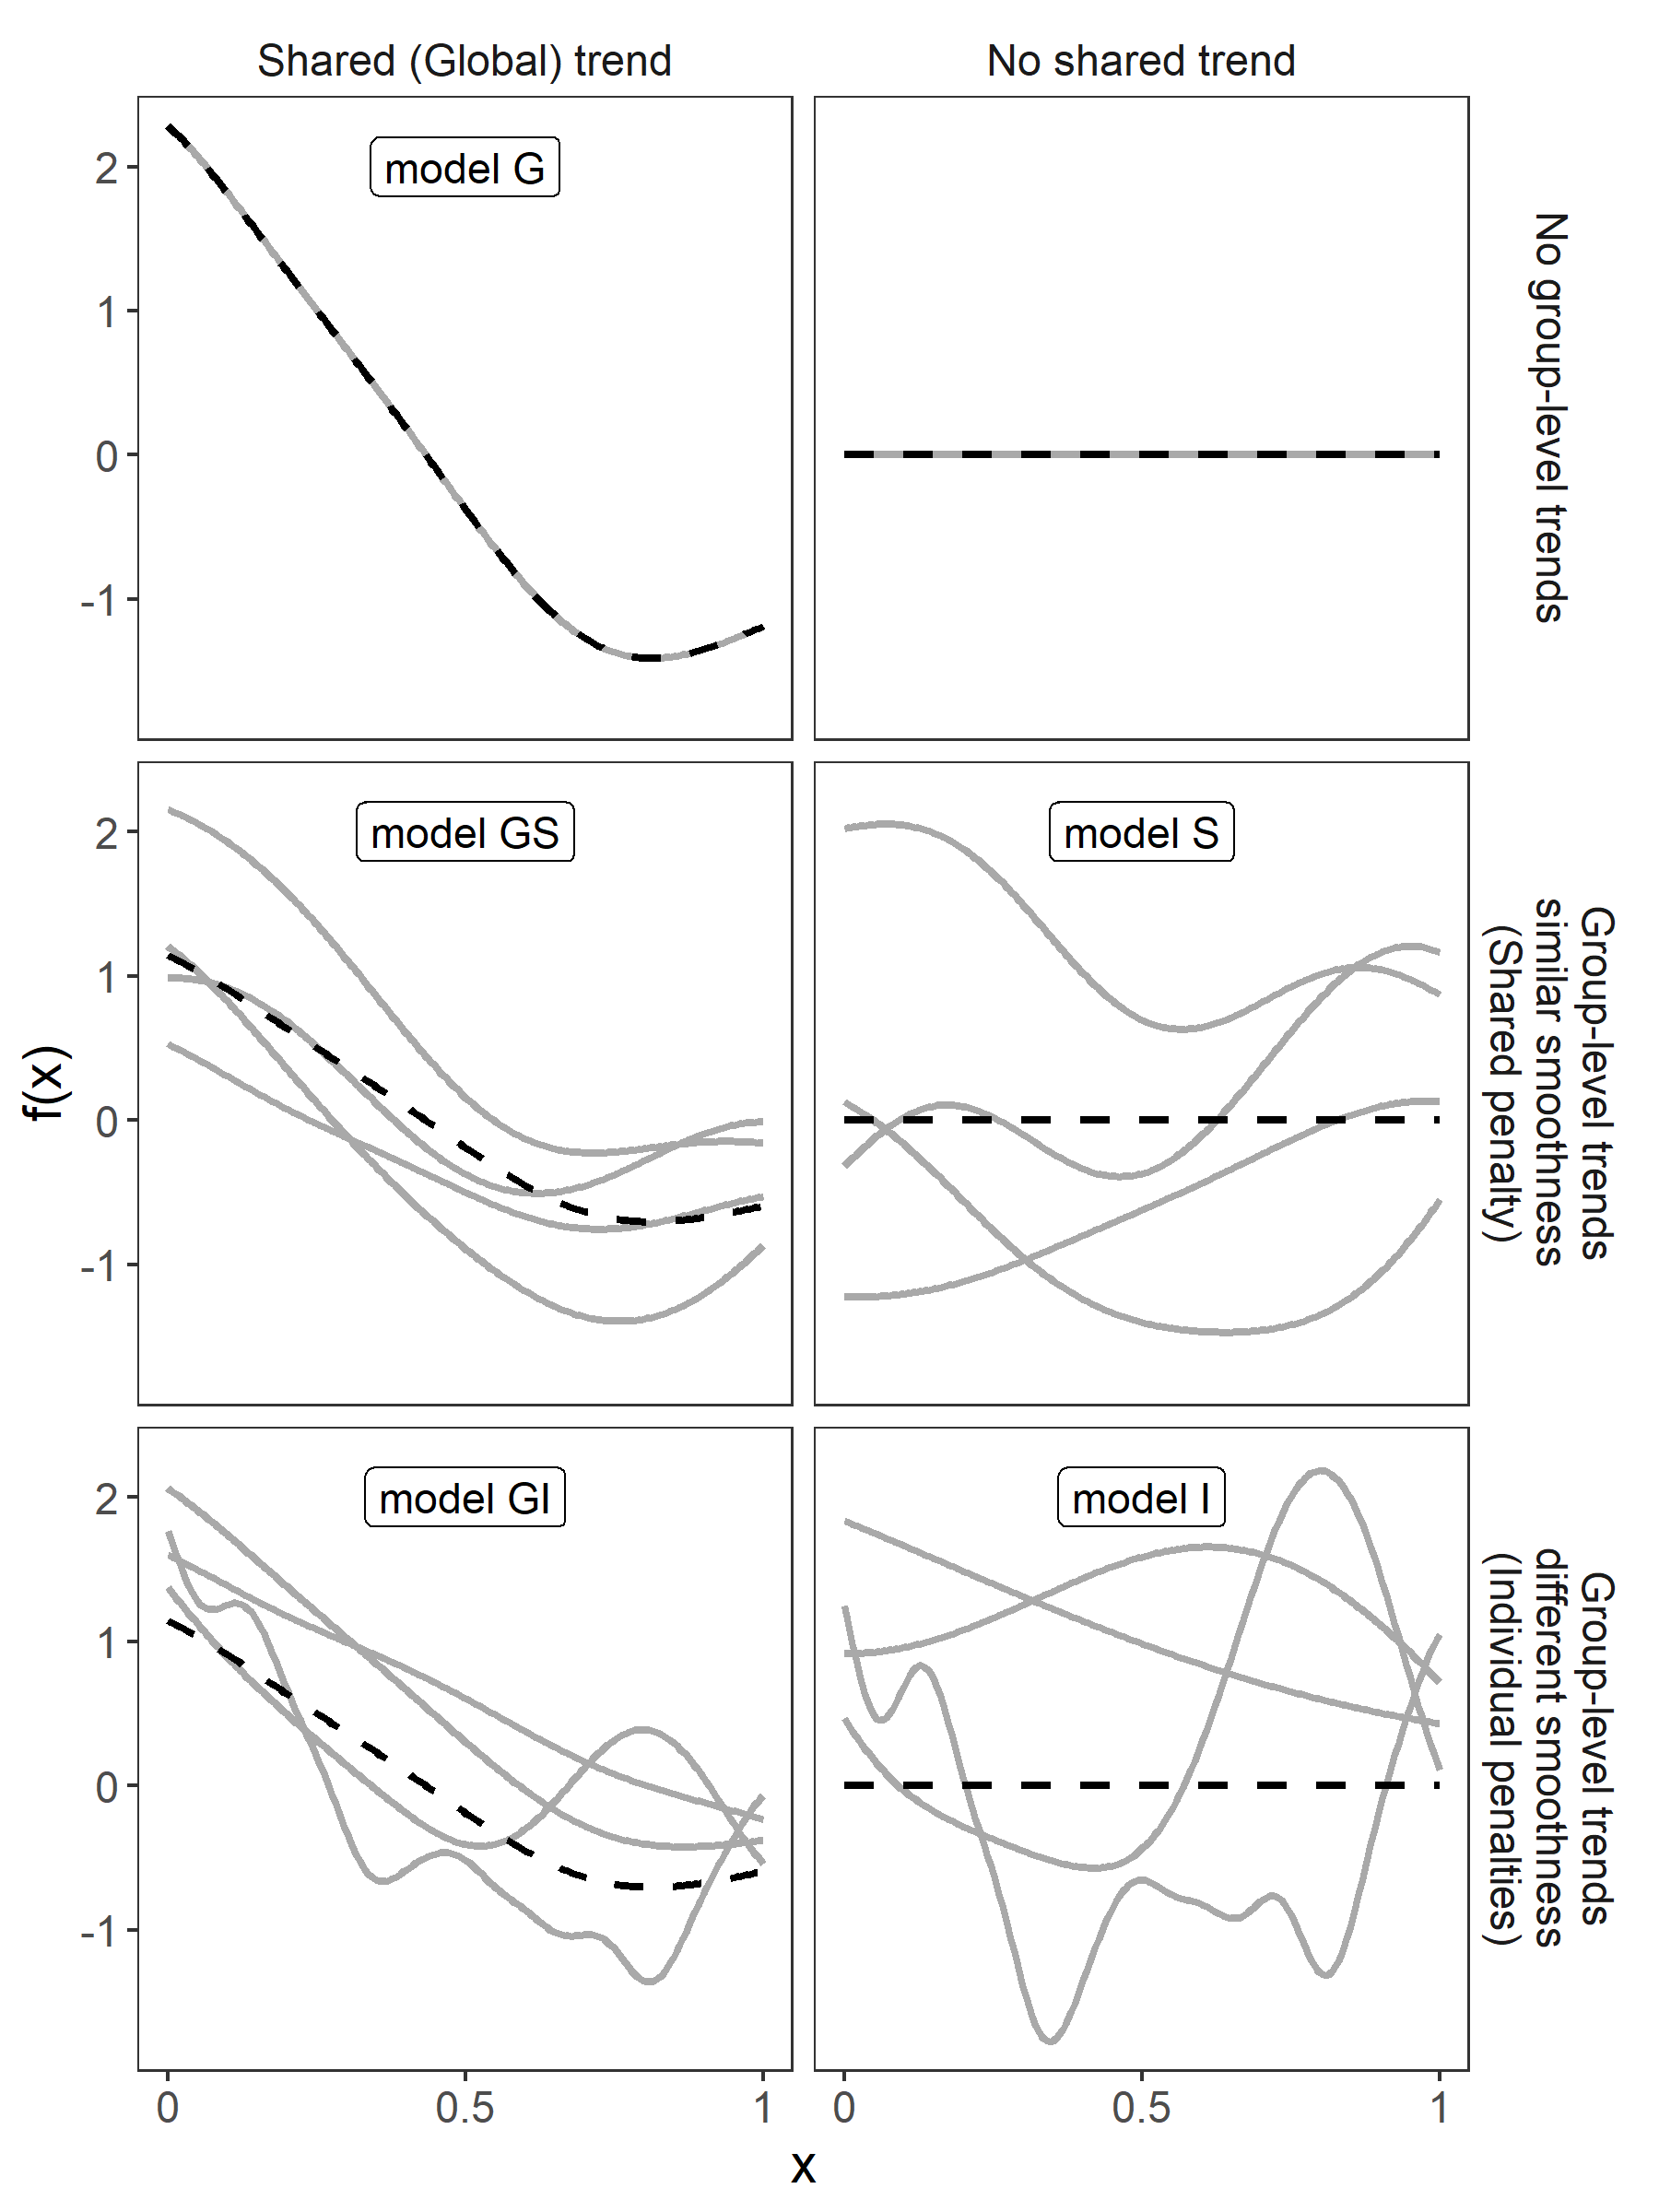
\includegraphics{../figures/alternate_models.png}
\caption{\label{fig:models}Alternate types of functional variation f(x)
that can be fitted with HGAMs. The dashed line indicates the average
function value for all groups, and each solid line indicates the
functional value at a given predictor value for an individual group
level. The null model (of no functional relationship between the
covariate and outcome, top right), is not explicitly assigned a model
number.}
\end{figure}

It is important to note that ``similar wiggliness'' and ``similar
shape'' are two distinct concepts; functions can have very similar
wiggliness but very different shapes. Wiggliness measures how quickly a
function changes across its range, and it is easy to construct two
functions that differ in shape but have the same wiggliness. For this
paper, we consider two functions to have similar shape if the average
squared distance between the functions is small (assuming the functions
have been scaled to have a mean value of zero across their ranges). This
definition is somewhat restricted; for instance, a cyclic function would
not be considered to have the same shape as a phase-shifted version of
the same function, nor would two normal distributions with the same mean
but different standard deviations. The benefit of this definition of
shape, however, is that it is straightforward to translate into
penalties akin to those described in section II. Figure
\ref{fig:models}, model \emph{S} illustrates the case where models have
different shapes. Similarly, two curves could have very similar overall
shape, but differ in their wiggliness. For instance, one function could
be equal to another plus a high-frequency oscillation term. Figure
\ref{fig:models}, model \emph{GI} illustrates this.

We will discuss the trade-offs between different models and guidelines
about when each of these models is appropriate in section V. The
remainder of this section will focus on how to specify each of these
five models using \textbf{mgcv}.

\subsection{Coding hierarchical GAMs in
R}\label{coding-hierarchical-gams-in-r}

Each of the models in Figure \ref{fig:models} can be coded
straightforwardly in \textbf{mgcv}. We will use two example datasets to
demonstrate how to code these models (see the supplemental code to
reproduce these examples):

A. The \texttt{CO2} dataset, available in R via the \textbf{datasets}
package. This data is from an experimental study by Potvin, Lechowicz \&
Tardif (1990) of CO\textsubscript{2} uptake in grasses under varying
concentrations of CO\textsubscript{2}, measuring how
concentration-uptake functions varied between plants from two locations
(Mississippi and Quebec) and two temperature treatments (chilled and
warm). Twelve plants were used and CO\textsubscript{2} uptake measured
at 7 CO\textsubscript{2} concentrations for each plant (figure
\ref{fig:vis_data}a). Here we will focus on how to use HGAMs to estimate
inter-plant variation in functional responses. This data set has been
modified from the default version available with R, to recode the
\texttt{Plant} variable as an unordered factor
\texttt{Plant\_uo}\footnote{Note that \textbf{mgcv} requires that
  grouping or categorical variables be coded as factors in R; it will
  raise an error message if passed data coded as characters. It is also
  important to know whether the factor is coded as ordered or unordered
  (see \texttt{?factor} for more details on this). This matters when
  fitting groupwise smoothers using the \texttt{by=} argument (as is
  used for fitting models \emph{GI} and \emph{I}, shown below). If the
  factor is unordered, \textbf{mgcv} will set up a model with one
  smoother for each grouping level. If the factor is ordered,
  \textbf{mgcv} will set any basis functions for the first grouping
  level to zero. In model \emph{GI} the ungrouped smoother will then
  correspond to the first grouping level, rather than the average
  functional response, and the group-specific smoothers will correspond
  to deviations from the first group. In model \emph{I}, using an
  ordered factor will result in the first group not having a smoother
  associated with it at all.}.

B. Data generated from a hypothetical study of bird movement along a
migration corridor, sampled throughout the year (see supplemental code).
This dataset consists of simulated sample records of numbers of observed
locations of 100 tagged individuals each from six species of bird, at
ten locations along a latitudinal gradient, with one observation taken
every four weeks. Counts were simulated randomly for each species in
each location and week by creating a species-specific migration curve
that gave the probability of finding an individual of a given species in
a given location, then simulated the distribution of individuals across
sites using a multinomial distribution, and subsampling that using a
binomial distribution to simulation observation error (i.e.~not every
bird present at a location would be detected). The data set
(\texttt{bird\_move}) consists of the variables \texttt{count},
\texttt{latitude}, \texttt{week} and \texttt{species} (figure
\ref{fig:vis_data}b). This example allows us to demonstrate how to fit
these models with interactions and with non-normal (count) data. The
true model used to generate this data was model \emph{GS}: a single
global function plus species-specific deviations around that global
function.

\begin{figure}
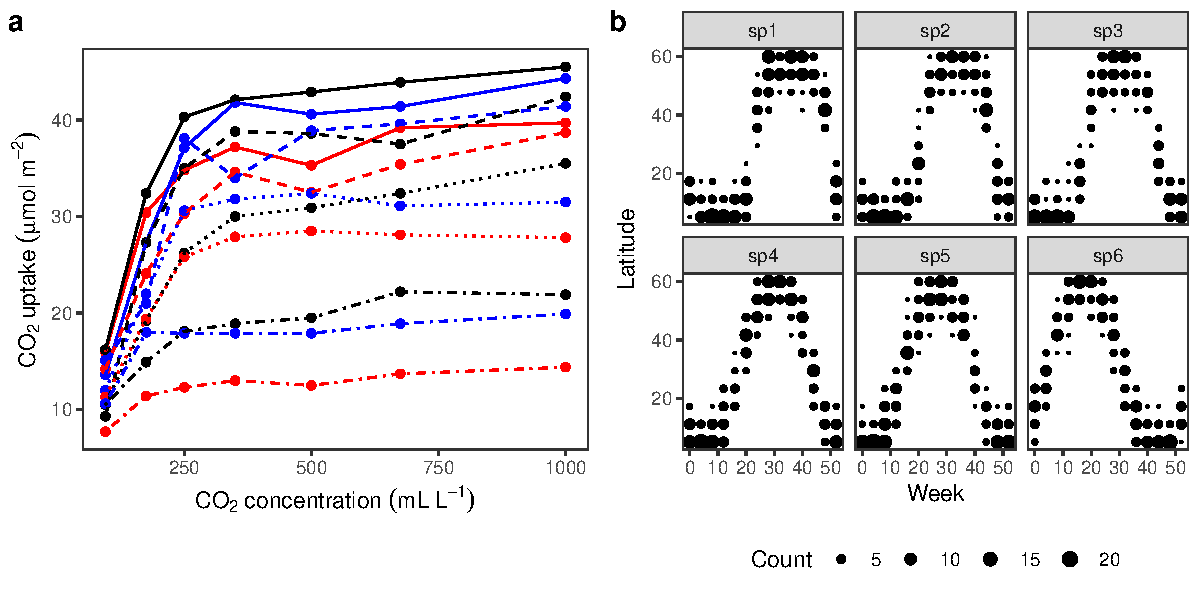
\includegraphics[width=\linewidth]{../figures/vis_data-1} \caption{\label{fig:vis_data}Example data sets used throughout section III. a) Grass $\text{CO}\textsubscript{2}$ uptake versus $\text{CO}\textsubscript{2}$ concentration for 12 individual plants. Color and linetype included to distinguish individual plant trends. b) Simulated data set of bird migration, with point size corresponding to weekly counts of 6 species along a latitudinal gradient (zeros excluded for clarity). }\label{fig:vis_data}
\end{figure}

Throughout the examples we use Restricted Maximum Likelihood (REML) to
estimate model coefficients and smoothing parameters. We strongly
recommend using either REML or marginal likelihood (ML) rather than the
default GCV criteria when fitting GAMs, for the reasons outlined in Wood
(2011). In each case some data processing and manipulation has been done
to obtain the graphics and results below. See supplemental code for
details on data processing steps. To illustrate plots, we will be using
the \texttt{draw} function from the \textbf{gratia} package; this
package was developed by one of the authors (Simpson, 2018) as a set of
tools to extend plotting and analysis of \textbf{mgcv} models. While
\textbf{mgcv} does have default plotting capabilities (through
\texttt{plot(\textless{}model\_name\textgreater{})}), \textbf{gratia}
expands these by creating \textbf{ggplot2} objects (Wickham, 2016) that
can be more easily extended and modified.

\subsubsection{\texorpdfstring{A single common (global) smoother for all
observations (Model
\emph{G})}{A single common (global) smoother for all observations (Model G)}}\label{a-single-common-global-smoother-for-all-observations-model-g}

We start with the simplest model we can in our framework and include
many details here to ensure that readers are comfortable with the
terminology and R functions we are going to use later.

For our \texttt{CO2} data set, we will model \(\log_e(\texttt{uptake})\)
as a function of two smoothers: a thin plate regression spline of
\(\log_e\)-concentration, and a random effect for plant to model
plant-specific intercepts. Mathematically:

\[
\log_e(\texttt{uptake}_i) = f(\log_e(\texttt{conc}_i)) + \zeta_\texttt{Plant\_uo} + \varepsilon_i
\]

where \(\zeta_\texttt{Plant\_uo}\) is the random effect for plant and
\(\varepsilon_i\) is a Gaussian error term. Here we assume that
\(\log_e(\texttt{uptake}_i)\) is normally distributed.

In R we can write our model as:

\begin{Shaded}
\begin{Highlighting}[]
\NormalTok{CO2_modG <-}\StringTok{ }\KeywordTok{gam}\NormalTok{(}\KeywordTok{log}\NormalTok{(uptake) }\OperatorTok{~}\StringTok{ }\KeywordTok{s}\NormalTok{(}\KeywordTok{log}\NormalTok{(conc), }\DataTypeTok{k=}\DecValTok{5}\NormalTok{, }\DataTypeTok{bs=}\StringTok{"tp"}\NormalTok{) }\OperatorTok{+}
\StringTok{                  }\KeywordTok{s}\NormalTok{(Plant_uo, }\DataTypeTok{k=}\DecValTok{12}\NormalTok{, }\DataTypeTok{bs=}\StringTok{"re"}\NormalTok{),}
                \DataTypeTok{data=}\NormalTok{CO2, }\DataTypeTok{method=}\StringTok{"REML"}\NormalTok{, }\DataTypeTok{family=}\StringTok{"gaussian"}\NormalTok{)}
\end{Highlighting}
\end{Shaded}

This is a common GAM structure, with a single smooth term for each
variable. Specifying the model is similar to specifying a GLM in R via
\texttt{glm()}, with the addition of \texttt{s()} terms to include
one-dimensional or isotropic multidimensional smoothers. The first
argument to \texttt{s()} are the terms to be smoothed, the type of
smoother to be used for the term is specified by the \texttt{bs}
argument, and the maximum number of basis functions is specified by
\texttt{k}. There are different defaults in \textbf{mgcv} for k,
depending on the type of smoother chosen; here we use a tprs smoother
(\texttt{bs="tp"}) for the concentration smoother, and set \texttt{k=5}
as there are only 7 separate values of concentration measured, so the
default \texttt{k=10} (for tprs) would be too high; further, setting
\texttt{k=5} saves on computational time (see section V). The random
effect smoother (\texttt{bs="re"}) that we used for the
\texttt{Plant\_uo} factor has a default \texttt{k} equal to the number
of levels in the grouping variable (here, 12). We specified
\texttt{k=12} just to make this connection apparent.

\begin{figure}
\centering
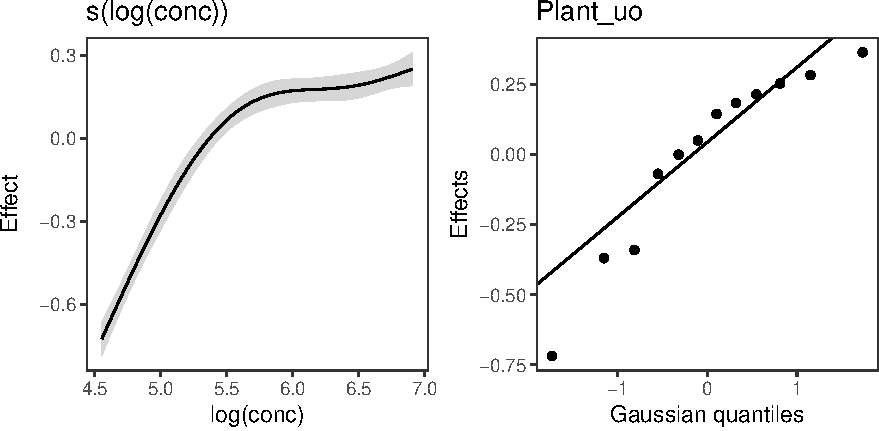
\includegraphics{../figures/co2_modG-1.pdf}
\caption{\label{fig:co2_modG}\textbf{gratia} plotting output for model
\emph{G} applied to the CO2 dataset. Left shows the smoother of
\(\log_e\) concentration and right plot shows a quantile-quantile plot
of the random effects against Gaussian quantiles, used to check the
appropriateness of the normal random effect assumption. Numbers in the
vertical axis of the left figure and the title of the right give the
effective degrees of freedom of the smoothers.}
\end{figure}

Figure \ref{fig:co2_modG} illustrates the output of \textbf{gratia}'s
\texttt{draw} function for \texttt{CO2\_modG}: the left panel shows the
estimated smoother for concentration, and the right shows a
quantile-quantile plot of the estimated random effects vs Gaussian
quantiles, which can be used to check our model.

Looking at the effects by term is useful, but we are often interested in
fitted values or predictions from our models. Using the built in
prediction functions with \textbf{mgcv}, we can estimate what the fitted
function (and uncertainty around it) should look like for each level, as
shown in Figure \ref{fig:co2_modG_predict} (see supplemental code for
more details on how to generate these predictions).

\begin{figure}
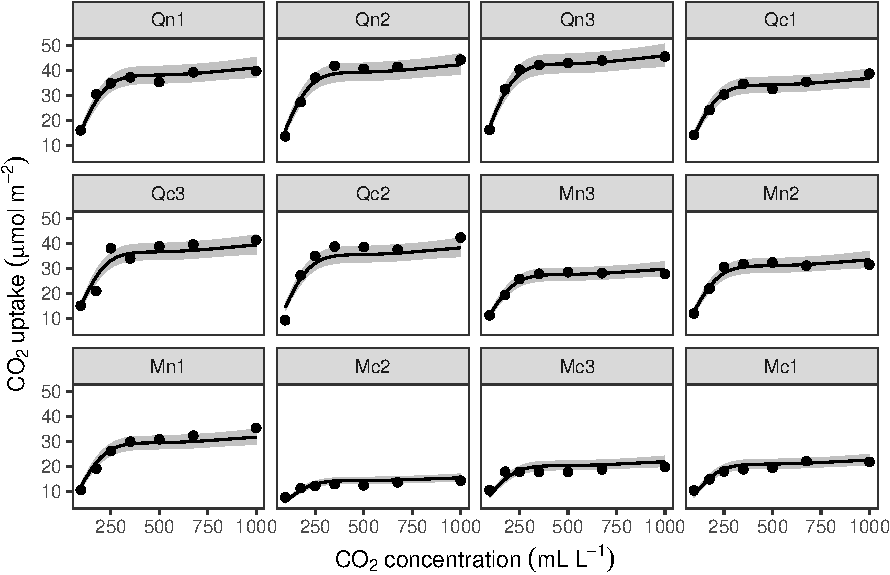
\includegraphics[width=\linewidth]{../figures/co2_modG_ggplot-1} \caption{\label{fig:co2_modG_predict} Predicted uptake function ($\pm$ 2 s.e.) for each plant, based on model *G* (a single global function for uptake plus a individual-level random effect intercept). Model predictions are for log-uptake, but are transformed here to show the fitted function on the original scale of the data.}\label{fig:co2_modG_ggplot}
\end{figure}

Examining these plots, we see that while functional responses among
plants are similar, some patterns are not captured by this model. For
instance, for plant Qc2, the model clearly underestimates CO2 uptake. A
model including individual differences in functional responses may
better explain variation.

For our bird example, we model the count of birds as a function of
location and time, including their interaction. For this we structure
the model as:

\[
\mathbb{E}(\texttt{count}_i) = \exp(f(\texttt{week}_i, \texttt{latitude}_i))
\]

where we assume that \(\texttt{count}_i \sim\text{Poisson}\). For the
smooth term, \(f\), we employ a tensor product of \texttt{latitude} and
\texttt{week}, using a thin plate regression spline (TPRS) for the
marginal latitude effect, and a cyclic cubic regression spline for the
marginal week effect to account for the cyclic nature of weekly effects
(we expect week 1 and week 52 to have very similar values)\footnote{The
  cyclic smoother requires that the start and end points of the cyclic
  variable are specified, via the \texttt{knots} argument; the smoother
  will have the exact same value at the start and end. In the absence of
  a specified start and end point, \texttt{gam} will assume the end
  points are the smallest and largest observed levels of the covariate
  (see \texttt{mgcv::smooth.construct.cc.smooth.spec} for more details).
  Note that in \texttt{bird\_modG} we have specified week 0 and week 52
  as the endpoints, as the first (week 1) and last weeks (week 52) of
  the year should not have exactly the same expected value.}, both
splines had basis complexity (\texttt{k}) of 10.

\begin{Shaded}
\begin{Highlighting}[]
\NormalTok{bird_modG <-}\StringTok{ }\KeywordTok{gam}\NormalTok{(count }\OperatorTok{~}\StringTok{ }\KeywordTok{te}\NormalTok{(week, latitude, }\DataTypeTok{bs=}\KeywordTok{c}\NormalTok{(}\StringTok{"cc"}\NormalTok{, }\StringTok{"tp"}\NormalTok{), }\DataTypeTok{k=}\KeywordTok{c}\NormalTok{(}\DecValTok{10}\NormalTok{, }\DecValTok{10}\NormalTok{)),}
                 \DataTypeTok{data=}\NormalTok{bird_move, }\DataTypeTok{method=}\StringTok{"REML"}\NormalTok{, }\DataTypeTok{family=}\StringTok{"poisson"}\NormalTok{,}
                 \DataTypeTok{knots =} \KeywordTok{list}\NormalTok{(}\DataTypeTok{week =} \KeywordTok{c}\NormalTok{(}\DecValTok{0}\NormalTok{, }\DecValTok{52}\NormalTok{)))}
\end{Highlighting}
\end{Shaded}

\begin{figure}
\centering
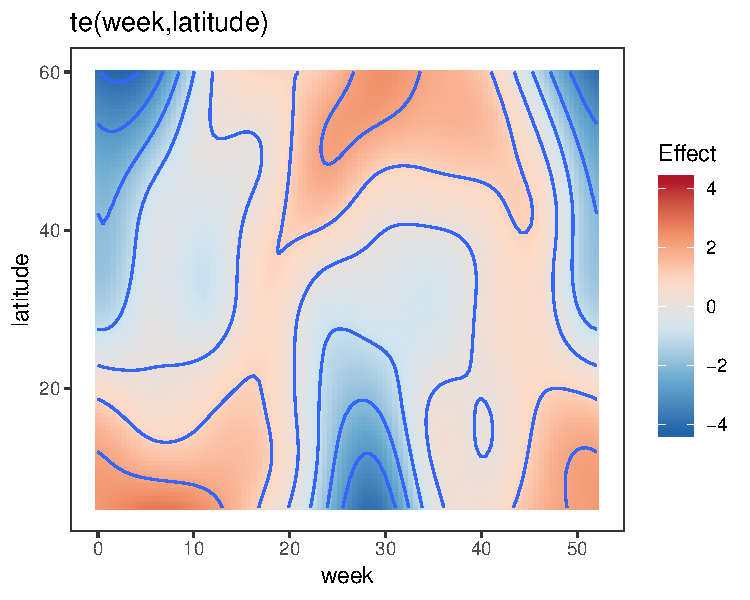
\includegraphics{../figures/bird_modG_plot-1.pdf}
\caption{\label{fig:bird_modG} Plot illustrating the average
log-abundance of all bird species at each latitude for each week, with
yellow colours indicating more individuals and red colours fewer.}
\end{figure}

Fig, \ref{fig:bird_modG} shows the default \texttt{draw(bird\_modG)}
plot for the week-by-latitude smoother. It shows birds starting at low
latitudes in the winter then migrating to high latitudes from the 10th
to 20th week, staying there for 15-20 weeks, then migrating back.
However, the plot also indicates a large amount of variability in the
timing of migration. The source of this variability is apparent when we
look at the timing of migration of each species (cf.~figure
\ref{fig:vis_data}b).

All six species in figure \ref{fig:vis_data}b show relatively precise
migration patterns, but they differ in the timing of when they leave
their winter grounds and the amount of time they spend at their summer
grounds. Averaging over all of this variation results in a relatively
imprecise (diffuse) estimate of migration timing (figure
\ref{fig:bird_modG}), and viewing species-specific plots of observed
versus predicted values (figure \ref{fig:bird-fitted-modG}), it is
apparent that the model fits some of the species better than others.
This model could potentially be improved by adding inter-group variation
in migration timing. The rest of this section will focus on how to model
this type of variation.

\begin{figure}
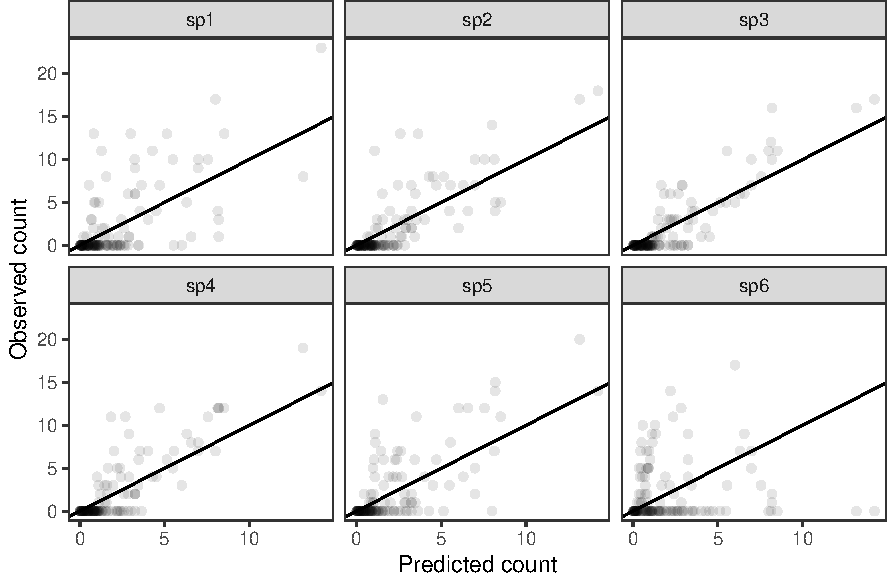
\includegraphics[width=\linewidth]{../figures/bird-fitted-modG-1} \caption{\label{fig:bird-fitted-modG}Observed counts by species versus predicted counts from \texttt{bird\_modG} (1-1 line added as reference). If our model fitted well we would expect that all species should show similiar patterns of dispersion around the 1-1 line (and as we are assuming the data is Poisson, the variance around the mean should equal the mean). Instead we see that variance around the predicted value is much higher for species 1 and 6.}\label{fig:bird-fitted-modG}
\end{figure}

\subsubsection{\texorpdfstring{A single common smoother plus group-level
smoothers that have the same wiggliness (model
\emph{GS})}{A single common smoother plus group-level smoothers that have the same wiggliness (model GS)}}\label{a-single-common-smoother-plus-group-level-smoothers-that-have-the-same-wiggliness-model-gs}

model \emph{GS} is a close analogue to a GLMM with varying slopes: all
groups have similar functional responses, but inter-group variation in
responses is allowed. This approach works by allowing each grouping
level to have its own functional response, but penalizing functions that
are too far from the average.

This can be coded in \textbf{mgcv} by explicitly specifying one term for
the global smoother (as in model \emph{G} above) then adding a second
smooth term specifying the group-level smooth terms, using a penalty
term that tends to draw these group-level smoothers to zero. For
one-dimensional smoothers, \textbf{mgcv} provides an explicit basis type
to do this, the factor-smoother interaction or \texttt{"fs"} basis (see
\texttt{?mgcv::factor.smooth.interaction} for details). This smoother
creates a copy of each set of basis functions for each level of the
grouping variable, but only estimates one smoothing parameter for all
groups. To ensure that all parts of the smoother can be shrunk towards
zero effect, each component of the penalty null space is given its own
penalty\footnote{As part of the penalty construction, each group will
  also have its own intercept (part of the penalized null space), so
  there is no need to add a separate term for group specific intercepts
  as we did in model \emph{G}.}.

We modify the previous \(\text{CO}_2\) model to incorporate group-level
smoothers as follows:

\[
\log_e(\texttt{uptake}_i) = f(\log_e(\texttt{conc}_i)) + f_{\texttt{Plant\_uo}_i}(\log_e(\texttt{conc}_i)) + \varepsilon_i
\]

where \(f_{\texttt{Plant\_uo}_i}(\log_e(\texttt{conc}_i))\) is the
smoother for concentration for the given plant. In R we then have:

\begin{Shaded}
\begin{Highlighting}[]
\NormalTok{CO2_modGS <-}\StringTok{ }\KeywordTok{gam}\NormalTok{(}\KeywordTok{log}\NormalTok{(uptake) }\OperatorTok{~}\StringTok{ }\KeywordTok{s}\NormalTok{(}\KeywordTok{log}\NormalTok{(conc), }\DataTypeTok{k=}\DecValTok{5}\NormalTok{, }\DataTypeTok{m=}\DecValTok{2}\NormalTok{) }\OperatorTok{+}\StringTok{ }
\StringTok{                  }\KeywordTok{s}\NormalTok{(}\KeywordTok{log}\NormalTok{(conc), Plant_uo, }\DataTypeTok{k=}\DecValTok{5}\NormalTok{,  }\DataTypeTok{bs=}\StringTok{"fs"}\NormalTok{, }\DataTypeTok{m=}\DecValTok{2}\NormalTok{),}
                \DataTypeTok{data=}\NormalTok{CO2, }\DataTypeTok{method=}\StringTok{"REML"}\NormalTok{)}
\end{Highlighting}
\end{Shaded}

\begin{figure}
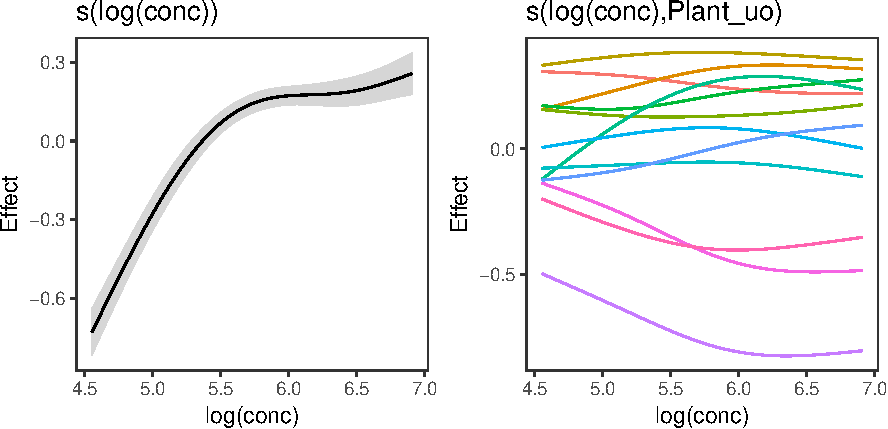
\includegraphics[width=\linewidth]{../figures/co2_modGS_plot-1} \caption{\label{fig:co2_modGS}Global function (left) and group-specific deviations from the global function (right) for \texttt{CO2\_modGS}}\label{fig:co2_modGS_plot}
\end{figure}

Figure \ref{fig:co2_modGS} shows the fitted smoothers for
\texttt{CO2\_modGS}. The plots of group-specific smoothers indicate that
plants differ not only in average log-uptake (which would correspond to
each plant having a straight line at different levels for the
group-level smoother), but differ slightly in the shape of their
functional responses. Figure \ref{fig:co2_modGS_pred} shows how the
global and group-specific smoothers combine to predict uptake rates for
individual plants. We see that, unlike in the single global smoother
case above, none of the curves deviate from the data systematically.

\begin{figure}
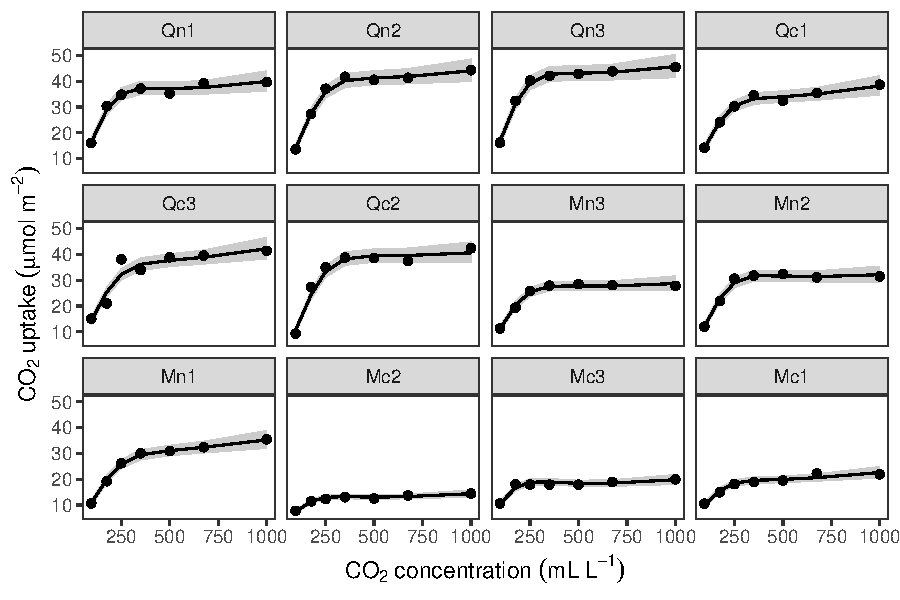
\includegraphics[width=\linewidth]{../figures/co2_modGS_ggplot-1} \caption{\label{fig:co2_modGS_pred}Predicted uptake values (lines) versus observed uptake for each plant, based on model *GS*.}\label{fig:co2_modGS_ggplot}
\end{figure}

The factor-smoother interaction-based approach mentioned above does not
work for higher-dimensional tensor product smoothers. Instead, the
group-specific term can be specified with a tensor product of the
continuous smoothers and a random effect for the grouping
parameter\footnote{As mentioned in section II, these terms can be
  specified either with \texttt{te()} or \texttt{t2()} terms. Using
  \texttt{t2} as above (with \texttt{full=TRUE}) is essentially a
  multivariate equivalent of the factor-smoother interaction; it
  requires more smooth terms than \texttt{te()}, but can be fit using
  other mixed effects software such as \textbf{lme4}, which is useful
  when fitting models with a large number of group levels (see Section V
  on computational issues for details).}. e.g.:
\texttt{y\ \textasciitilde{}\ te(x1,\ x2,\ bs="tp",\ m=2)\ +\ t2(x1,\ x2,\ fac,\ bs=c("tp","tp","re"),\ m=2,\ full=TRUE)}.
We illustrate this approach below on the bird migration data.

\begin{Shaded}
\begin{Highlighting}[]
\NormalTok{bird_modGS <-}\StringTok{ }\KeywordTok{gam}\NormalTok{(count }\OperatorTok{~}\StringTok{ }\KeywordTok{te}\NormalTok{(week, latitude, }\DataTypeTok{bs=}\KeywordTok{c}\NormalTok{(}\StringTok{"cc"}\NormalTok{, }\StringTok{"tp"}\NormalTok{),}
                            \DataTypeTok{k=}\KeywordTok{c}\NormalTok{(}\DecValTok{10}\NormalTok{, }\DecValTok{10}\NormalTok{), }\DataTypeTok{m=}\DecValTok{2}\NormalTok{) }\OperatorTok{+}
\StringTok{                   }\KeywordTok{t2}\NormalTok{(week, latitude, species, }\DataTypeTok{bs=}\KeywordTok{c}\NormalTok{(}\StringTok{"cc"}\NormalTok{, }\StringTok{"tp"}\NormalTok{, }\StringTok{"re"}\NormalTok{),}
                      \DataTypeTok{k=}\KeywordTok{c}\NormalTok{(}\DecValTok{10}\NormalTok{, }\DecValTok{10}\NormalTok{, }\DecValTok{6}\NormalTok{), }\DataTypeTok{m=}\DecValTok{2}\NormalTok{, }\DataTypeTok{full=}\OtherTok{TRUE}\NormalTok{),}
                 \DataTypeTok{data=}\NormalTok{bird_move, }\DataTypeTok{method=}\StringTok{"REML"}\NormalTok{, }\DataTypeTok{family=}\StringTok{"poisson"}\NormalTok{, }
                 \DataTypeTok{knots =} \KeywordTok{list}\NormalTok{(}\DataTypeTok{week =} \KeywordTok{c}\NormalTok{(}\DecValTok{0}\NormalTok{, }\DecValTok{52}\NormalTok{)))}
\end{Highlighting}
\end{Shaded}

\begin{figure}
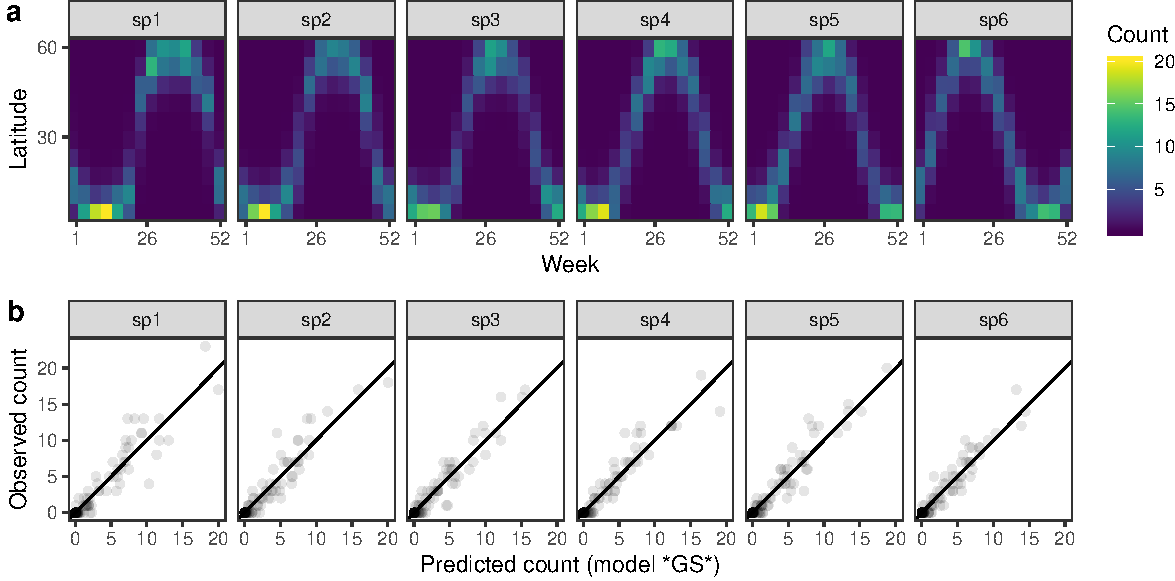
\includegraphics[width=\linewidth]{../figures/bird_modGS_ggplot-1} \caption{\label{fig:bird_modGS}a) Predicted migration paths for each species based on \texttt{bird\_modGS}, with lighter colors corresponding to higher predicted counts. b) Observed counts versus predictions from \texttt{bird\_modGS}.}\label{fig:bird_modGS_ggplot}
\end{figure}

Model \emph{GS} is able to effectively capture the observed patterns of
interspecific variation in migration behaviour (figure
\ref{fig:bird_modGS}a). It shows a much tighter fit between observed and
predicted values, as well as less evidence of over-dispersion in some
species compared to model \emph{G} (figure \ref{fig:bird_modGS}b).

\subsubsection{\texorpdfstring{A single common smoother plus group-level
smoothers with differing wiggliness (Model
\emph{GI})}{A single common smoother plus group-level smoothers with differing wiggliness (Model GI)}}\label{a-single-common-smoother-plus-group-level-smoothers-with-differing-wiggliness-model-gi}

This model class is very similar to model \emph{GS}, but we now allow
each group-specific smoother to have its own smoothing parameter and
hence its own level of wiggliness. This increases the computational cost
of the model (as there are more smoothing parameters to estimate), and
means that the only information shared between groups is through the
global smoother, the common error term, and through the random effect
for group-level intercepts (if used). This is useful if different groups
differ substantially in how wiggly they are.

Fitting a separate smoother (with its own penalties) can be done in
\textbf{mgcv} by using the \texttt{by} argument in the \texttt{s()} and
\texttt{te()} (and related) functions. Therefore, we can code the
formula for this model as:

\begin{Shaded}
\begin{Highlighting}[]
\NormalTok{y }\OperatorTok{~}\StringTok{ }\KeywordTok{s}\NormalTok{(x, }\DataTypeTok{bs=}\StringTok{"tp"}\NormalTok{) }\OperatorTok{+}\StringTok{ }\KeywordTok{s}\NormalTok{(x, }\DataTypeTok{by=}\NormalTok{fac, }\DataTypeTok{m=}\DecValTok{1}\NormalTok{, }\DataTypeTok{bs=}\StringTok{"tp"}\NormalTok{) }\OperatorTok{+}\StringTok{ }\KeywordTok{s}\NormalTok{(fac, }\DataTypeTok{bs=}\StringTok{"re"}\NormalTok{)}
\end{Highlighting}
\end{Shaded}

Note two major differences here from how model \emph{GS} was specified:

\begin{enumerate}
\def\labelenumi{\arabic{enumi}.}
\tightlist
\item
  We explicitly include a random effect for the intercept (the
  \texttt{bs="re"} term), as group-specific intercepts are not
  incorporated into factor \texttt{by} variable smoothers (as would be
  the case with a factor smoother or a tensor product random effect).
\item
  We specify \texttt{m=1} instead of \texttt{m=2} for the groupwise
  smoothers, which means the marginal TPRS basis for this term will
  penalize the squared 1st derivative of the function, rather than the
  second derivative. This, also, reduces co-linearity between the global
  smoother and the group-specific terms which occasionally leads to high
  uncertainty around the global smoother (see section V for more
  details). TPRS with \texttt{m=1} have a more restricted null space
  than m=2 smoothers, so should not be as collinear with the global
  smoother (Wieling et al., 2016; Baayen et al., 2018). We have observed
  that this is much more of an issue when fitting model \emph{GI}
  compared to model \emph{GS}.
\end{enumerate}

We modify the \texttt{CO2} model to follow this approach like so:

\begin{Shaded}
\begin{Highlighting}[]
\NormalTok{CO2_modGI <-}\StringTok{ }\KeywordTok{gam}\NormalTok{(}\KeywordTok{log}\NormalTok{(uptake) }\OperatorTok{~}\StringTok{ }\KeywordTok{s}\NormalTok{(}\KeywordTok{log}\NormalTok{(conc), }\DataTypeTok{k=}\DecValTok{5}\NormalTok{, }\DataTypeTok{m=}\DecValTok{2}\NormalTok{, }\DataTypeTok{bs=}\StringTok{"tp"}\NormalTok{) }\OperatorTok{+}
\StringTok{                  }\KeywordTok{s}\NormalTok{(}\KeywordTok{log}\NormalTok{(conc), }\DataTypeTok{by=}\NormalTok{Plant_uo, }\DataTypeTok{k=}\DecValTok{5}\NormalTok{, }\DataTypeTok{m=}\DecValTok{1}\NormalTok{, }\DataTypeTok{bs=}\StringTok{"tp"}\NormalTok{) }\OperatorTok{+}
\StringTok{                  }\KeywordTok{s}\NormalTok{(Plant_uo, }\DataTypeTok{bs=}\StringTok{"re"}\NormalTok{, }\DataTypeTok{k=}\DecValTok{12}\NormalTok{),}
                \DataTypeTok{data=}\NormalTok{CO2, }\DataTypeTok{method=}\StringTok{"REML"}\NormalTok{)}
\end{Highlighting}
\end{Shaded}

\begin{figure}
\centering
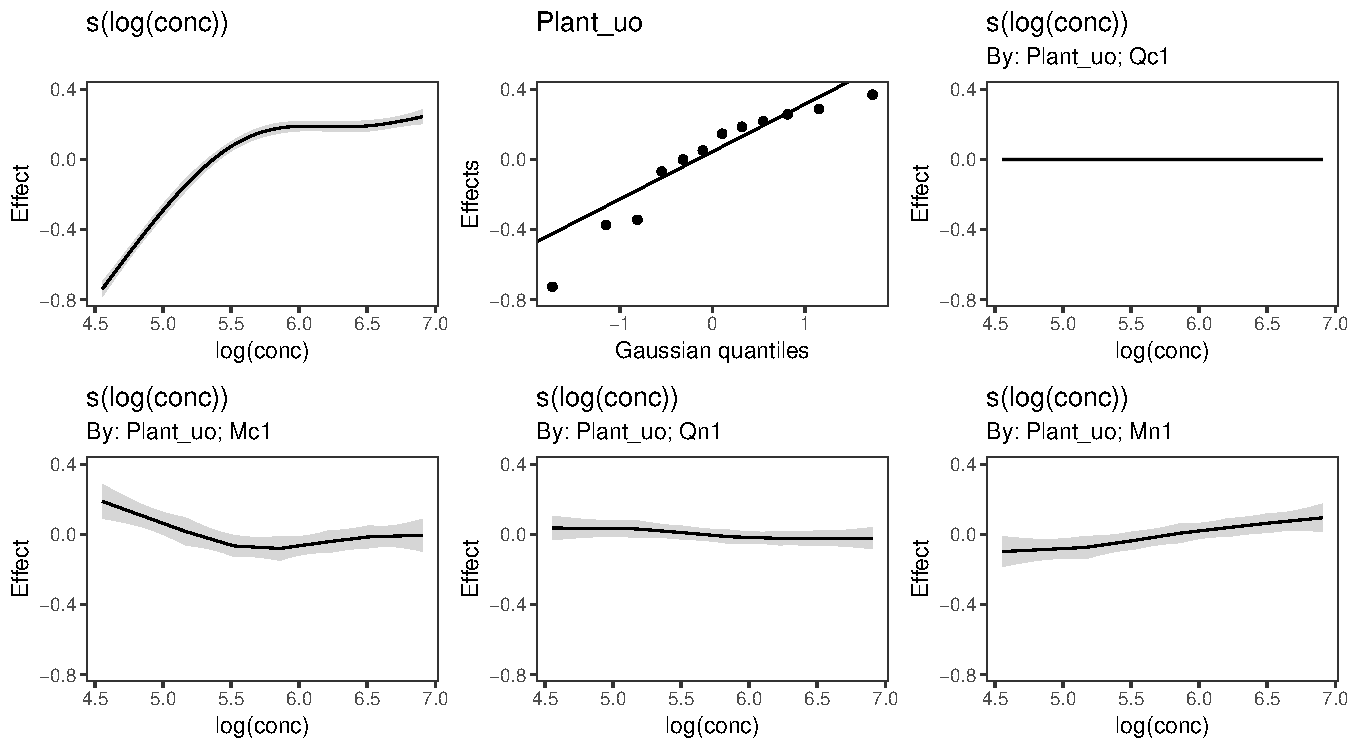
\includegraphics{../figures/modGI_CO2-1.pdf}
\caption{\label{fig:co2_modGI}Functional relationships for the CO2 data
estimated for model \emph{GI}. Top left: the global smoother; Top
middle: species-specific random effect intercepts. The remaining plots
are a selected subset of the plant-specific smoothers, indicating how
the functional response of that plant differs from the global smoother.}
\end{figure}

Figure \ref{fig:co2_modGI} shows a subsample of the group-specific
smoothers from this model. It is apparent from this that some groups
(e.g. \texttt{Qc1}) have very similar shapes to the global smoother
(differing only in intercept), others do differ from the global trend,
with higher uptake at low concentrations and lower uptake at higher
concentrations (e.g. \texttt{Mc1}, \texttt{Qn1}), or the reverse pattern
(e.g. \texttt{Mn1}).

Using model \emph{GI} with higher-dimensional data is also
straightforward; \texttt{by} terms work just as well in tensor-product
smoothers as they do with isotropic smoothers. We can see this with our
bird model:

\begin{Shaded}
\begin{Highlighting}[]
\NormalTok{bird_modGI <-}\StringTok{ }\KeywordTok{gam}\NormalTok{(count }\OperatorTok{~}\StringTok{ }\NormalTok{species }\OperatorTok{+}
\StringTok{                   }\KeywordTok{te}\NormalTok{(week, latitude, }\DataTypeTok{bs=}\KeywordTok{c}\NormalTok{(}\StringTok{"cc"}\NormalTok{, }\StringTok{"tp"}\NormalTok{),}
                      \DataTypeTok{k=}\KeywordTok{c}\NormalTok{(}\DecValTok{10}\NormalTok{, }\DecValTok{10}\NormalTok{), }\DataTypeTok{m=}\DecValTok{2}\NormalTok{) }\OperatorTok{+}
\StringTok{                   }\KeywordTok{te}\NormalTok{(week, latitude, }\DataTypeTok{by=}\NormalTok{species, }\DataTypeTok{bs=} \KeywordTok{c}\NormalTok{(}\StringTok{"cc"}\NormalTok{, }\StringTok{"tp"}\NormalTok{),}
                      \DataTypeTok{k=}\KeywordTok{c}\NormalTok{(}\DecValTok{10}\NormalTok{, }\DecValTok{10}\NormalTok{), }\DataTypeTok{m=}\DecValTok{1}\NormalTok{),}
                 \DataTypeTok{data=}\NormalTok{bird_move, }\DataTypeTok{method=}\StringTok{"REML"}\NormalTok{, }\DataTypeTok{family=}\StringTok{"poisson"}\NormalTok{,}
                 \DataTypeTok{knots =} \KeywordTok{list}\NormalTok{(}\DataTypeTok{week =} \KeywordTok{c}\NormalTok{(}\DecValTok{0}\NormalTok{, }\DecValTok{52}\NormalTok{)))}
\end{Highlighting}
\end{Shaded}

As above, we have set (\texttt{m=1}) for the latitude marginal effect to
avoid issues of collinearity between the global and groupwise smoother.
Note that switching \texttt{m=1} to \texttt{m=2} does not have any
effect on the marginal basis for \texttt{week}, where we are using a
cyclic smoother instead of a tprs.

The fitted model for \texttt{bird\_modGI} is visually indistinguishable
from \texttt{bird\_modGS} (figure \ref{fig:bird_modGS}) so we do not
illustrate it here.

\subsubsection{\texorpdfstring{Models without global smoothers (models
\emph{S} and
\emph{I})}{Models without global smoothers (models S and I)}}\label{models-without-global-smoothers-models-s-and-i}

We can modify the above models to exclude the global term (which is
generally faster; see section V). When we do not model the global term,
we are allowing each factor to be different, though there may be some
similarities in the shape of the functions.

\paragraph{\texorpdfstring{Model \emph{S}:}{Model S:}}\label{model-s}

Model \emph{S} (shared smoothers) is simply model \emph{GS} without the
global smoother; this type of model takes the form:
\texttt{y\textasciitilde{}s(x,\ fac,\ bs="fs")} or
\texttt{y\textasciitilde{}te(x1,\ x2,\ fac,\ bs=c("tp",\ "tp",\ "re")}
in \texttt{mgcv}. This model assumes all groups have the same
smoothness, but that the individual shapes of the smooth terms are not
related. Here we just show how to code these models; plotting them works
in the same way as for models \emph{G},\emph{GS}, and \emph{GI} above,
the plots for these datasets are very similar to the plots for model
\emph{GS}. This will not always be the case; if in a given study there
are very few data points in each grouping level (relative to the
strength of the functional relationship of interest), estimates from
model \emph{S} will typically be much more variable than from model
\emph{GS}, as there is no way for the model to share information on
function shape between grouping levels without the global smoother. See
section V on computational issues for more on how to choose between
different models.

\begin{Shaded}
\begin{Highlighting}[]
\NormalTok{CO2_modS <-}\StringTok{ }\KeywordTok{gam}\NormalTok{(}\KeywordTok{log}\NormalTok{(uptake) }\OperatorTok{~}\StringTok{ }\KeywordTok{s}\NormalTok{(}\KeywordTok{log}\NormalTok{(conc), Plant_uo, }\DataTypeTok{k=}\DecValTok{5}\NormalTok{, }\DataTypeTok{bs=}\StringTok{"fs"}\NormalTok{, }\DataTypeTok{m=}\DecValTok{2}\NormalTok{),}
                \DataTypeTok{data=}\NormalTok{CO2, }\DataTypeTok{method=}\StringTok{"REML"}\NormalTok{)}

\NormalTok{bird_modS <-}\StringTok{ }\KeywordTok{gam}\NormalTok{(count }\OperatorTok{~}\StringTok{ }\KeywordTok{t2}\NormalTok{(week, latitude, species, }\DataTypeTok{bs=}\KeywordTok{c}\NormalTok{(}\StringTok{"cc"}\NormalTok{, }\StringTok{"tp"}\NormalTok{, }\StringTok{"re"}\NormalTok{),}
                            \DataTypeTok{k=}\KeywordTok{c}\NormalTok{(}\DecValTok{10}\NormalTok{, }\DecValTok{10}\NormalTok{, }\DecValTok{6}\NormalTok{), }\DataTypeTok{m=}\KeywordTok{c}\NormalTok{(}\DecValTok{2}\NormalTok{, }\DecValTok{2}\NormalTok{, }\DecValTok{2}\NormalTok{)),}
                 \DataTypeTok{data=}\NormalTok{bird_move, }\DataTypeTok{method=}\StringTok{"REML"}\NormalTok{, }\DataTypeTok{family=}\StringTok{"poisson"}\NormalTok{,}
                 \DataTypeTok{knots =} \KeywordTok{list}\NormalTok{(}\DataTypeTok{week =} \KeywordTok{c}\NormalTok{(}\DecValTok{0}\NormalTok{, }\DecValTok{52}\NormalTok{)))}
\end{Highlighting}
\end{Shaded}

\paragraph{\texorpdfstring{Model \emph{I}:}{Model I:}}\label{model-i}

Model \emph{I} is simply model \emph{GI} without the first term:
\texttt{y\textasciitilde{}fac+s(x,\ by=fac)} or
\texttt{y\textasciitilde{}fac+te(x1,x2,\ by=fac)} (as above, plots are
very similar to model \emph{GI}).

\begin{Shaded}
\begin{Highlighting}[]
\NormalTok{CO2_modI <-}\StringTok{ }\KeywordTok{gam}\NormalTok{(}\KeywordTok{log}\NormalTok{(uptake) }\OperatorTok{~}\StringTok{ }\KeywordTok{s}\NormalTok{(}\KeywordTok{log}\NormalTok{(conc), }\DataTypeTok{by=}\NormalTok{Plant_uo, }\DataTypeTok{k=}\DecValTok{5}\NormalTok{, }\DataTypeTok{bs=}\StringTok{"tp"}\NormalTok{, }\DataTypeTok{m=}\DecValTok{2}\NormalTok{) }\OperatorTok{+}
\StringTok{                              }\KeywordTok{s}\NormalTok{(Plant_uo, }\DataTypeTok{bs=}\StringTok{"re"}\NormalTok{, }\DataTypeTok{k=}\DecValTok{12}\NormalTok{),}
                \DataTypeTok{data=}\NormalTok{ CO2, }\DataTypeTok{method=}\StringTok{"REML"}\NormalTok{)}


\NormalTok{bird_modI <-}\StringTok{ }\KeywordTok{gam}\NormalTok{(count }\OperatorTok{~}\StringTok{ }\NormalTok{species }\OperatorTok{+}\StringTok{ }
\StringTok{                   }\KeywordTok{te}\NormalTok{(week, latitude, }\DataTypeTok{by=}\NormalTok{species, }\DataTypeTok{bs=} \KeywordTok{c}\NormalTok{(}\StringTok{"cc"}\NormalTok{, }\StringTok{"tp"}\NormalTok{), }
                      \DataTypeTok{k=}\KeywordTok{c}\NormalTok{(}\DecValTok{10}\NormalTok{, }\DecValTok{10}\NormalTok{), }\DataTypeTok{m=}\DecValTok{2}\NormalTok{),}
                 \DataTypeTok{data=}\NormalTok{bird_move, }\DataTypeTok{method=}\StringTok{"REML"}\NormalTok{, }\DataTypeTok{family=}\StringTok{"poisson"}\NormalTok{,}
                 \DataTypeTok{knots =} \KeywordTok{list}\NormalTok{(}\DataTypeTok{week =} \KeywordTok{c}\NormalTok{(}\DecValTok{0}\NormalTok{, }\DecValTok{52}\NormalTok{)))}
\end{Highlighting}
\end{Shaded}

\subsection{Comparing different HGAM
specifications}\label{comparing-different-hgam-specifications}

These models can be compared using standard model comparison tools.
Model \emph{GS} and model \emph{GI} will generally be nested in model
\emph{G} (depending on how each model is specified) so comparisons using
generalized likelihood ratio tests (GLRTs) may be used to test if
groupwise smoothers are necessary. However, we do not currently
recommend this method. There is not sufficient theory on how accurate
parametric p-values are for comparing these models; there is uncertainty
about what degrees of freedom to assign to models with varying
smoothness, and slightly different model specifications may not result
in nested models. (See Wood (2017a) Section 6.12.4 and
\texttt{?mgcv::anova.gam} for more discussion on using GLRTs to compare
GAMs.)

Comparing models based on AIC is a more robust approach to comparing the
different model structures. There is well-developed theory of how to
include effects of penalization and smoothing parameter uncertainty when
estimating the model complexity penalty for AIC (Wood, Pya \& Säfken,
2016). We demonstrate this approach in Table \ref{tab:AIC_table_kable}.
Using AIC, there is strong support for including among-group functional
variability for both the CO2 dataset and the \texttt{bird\_move} dataset
(compare models \emph{G} versus all other models). For the CO2 dataset
(Table \ref{tab:AIC_table_kable}A), there is relatively strong evidence
that there is more inter-group variability in smoothness than model
\emph{GS} allows, and weaker evidence that model \emph{S} or \emph{I}
(separate smoothers for all plants) show the best fit.

For the \texttt{bird\_move} dataset (Table \ref{tab:AIC_table_kable}B),
model \emph{GS} (global smoother plus group-level smoothers with a
shared penalty) gives the best fit for all models including a global
smooth (which is good as we simulated the data from a model with this
structure!). However, model \emph{S} (without a global term) still fits
this data better than model \emph{GS} based on AIC. This highlights an
issue with AIC for selecting between models with and without a global
smooth: as it is possible to fully recreate the global term by just
allowing each group-level smoother to have a similiar shape to one
another (that is, the global term is totally concurve with the
group-level smoothers; see section V) model selection criteria such as
AIC may indicate that the extra parameters required to fit the global
smoother are unnecessary.

\begin{table}[t]

\caption{\label{tab:AIC_table_kable}AIC table comparing model fits for example datasets}
\centering
\begin{tabular}{lrrr}
\toprule
Model & df & AIC & deltaAIC\\
\midrule
\addlinespace[0.3em]
\multicolumn{4}{l}{\textbf{A. CO2 models}}\\
\hspace{1em}CO2\_modG & 17 & -119 & 101\\
\hspace{1em}CO2\_modGS & 39 & -199 & 22\\
\hspace{1em}CO2\_modGI & 42 & -216 & 4\\
\hspace{1em}CO2\_modS & 53 & -219 & 1\\
\hspace{1em}CO2\_modI & 56 & -220 & 0\\
\addlinespace[0.3em]
\multicolumn{4}{l}{\textbf{B. bird\_move models}}\\
\hspace{1em}bird\_modG & 51 & 3374 & 1820\\
\hspace{1em}bird\_modGS & 140 & 1554 & 0\\
\hspace{1em}bird\_modGI & 208 & 1682 & 128\\
\hspace{1em}bird\_modS & 130 & 1555 & 1\\
\hspace{1em}bird\_modI & 200 & 1634 & 80\\
\bottomrule
\end{tabular}
\end{table}

Given this issue with selecting global terms, we strongly recommend not
selecting models based purely on AIC. Instead, model selection should be
based on expert subject knowledge about the system, computational time,
and most importantly, the inferential goals of the study. Table
\ref{tab:AIC_table_kable}A indicates that models \emph{S} and \emph{I}
(which do not have a global function) fit the \texttt{CO2} data better
than models with a global function, and that model \emph{S} fits the
\texttt{bird\_move} data better than model \emph{GS}. However, it is the
shape of the global function that we are actually interested in here, as
models \emph{S} and \emph{I} cannot be used to predict the
concentration-uptake relationship for plants that are not part of the
training set, or the average migration path for birds. The same
consideration holds when choosing between model \emph{GS} and \emph{GI}:
while model \emph{GI} fits the \texttt{CO2} data better than model
\emph{GS} (as measured by AIC), model \emph{GS} can be used to simulate
functional variation for unobserved group levels, whereas this is not
possible within the framework of model \emph{GI}. The next section works
through two examples to show how to choose between different models, and
section V discusses these and other model fitting issues in more depth.

It also is important to recognize that AIC, like any function of the
data, is a random variable and should be expected to have some sampling
error (Forster \& Sober, 2011). In cases when the goal is to select the
model that has the best predictive ability, we recommend holding some
fraction of the data out prior to the analysis and comparing how well
different models fit that data or using \(k\)-fold cross validation as a
more accurate guide to how well a given model may predict out of sample.
Predictive accuracy may also be substantially improved by averaging over
multiple models (Dormann et al., 2018).

\FloatBarrier

\section{IV: Examples}\label{iv-examples}

We now demonstrate two worked examples on one data set to highlight how
to use HGAMs in practice, and to illustrate how to fit, test, and
visualize each model. We will demonstrate how to use these models to fit
community data, to show when using a global trend may or may not be
justified, and to illustrate how to use these models to fit seasonal
time series.

For these examples, data are from a long-term study in seasonal dynamics
of zooplankton, collected by the Richard Lathrop. The data were
collected from a chain of lakes in Wisconsin (Mendota, Monona, Kegnonsa,
and Waubesa) approximately bi-weekly from 1976 to 1994. They consist of
samples of the zooplankton communities, taken from the deepest point of
each lake via vertical tow. The data are provided by the Wisconsin
Department of Natural Resources and their collection and processing are
fully described in Lathrop (2000).

Zooplankton in temperate lakes often undergo seasonal cycles, where the
abundance of each species fluctuates up and down across the course of
the year, with each species typically showing a distinct pattern of
seasonal cycles. The inferential aims of these examples are to
\emph{(i)} estimate variability in seasonality among species in the
community in a single lake (Mendota), and \emph{(ii)} estimate
among-lake variability for the most abundant taxon in the sample
(\emph{Daphnia mendotae}) across the four lakes. To enable evaluation of
out-of-sample performance, we split the data into testing and training
sets. As there are multiple years of data, we used data from the even
years to fit (train) models, and the odd years to test the fit.

Each record consists of counts of a given zooplankton taxon taken from a
subsample from a single vertical net tow, which was then scaled to
account for the relative volume of subsample versus the whole net sample
and the area of the net tow and rounded to the nearest 1000 to give
estimated population density per \(m^2\) for each taxon at each point in
time in each sampled lake. As this meant that data were not counts, and
observed densities spanned four orders of magnitude, we modelled density
using a Gamma distribution with a log-link. For any net tow sample where
a given taxon was not observed, we set that taxon's density to 1000 (the
minimum possible sample size)\footnote{A more appropriate model for this
  data would be to assume that density is \emph{left censored}, where
  1000 is treated as a threshold which the data may lie below, but it is
  not possible to measure lower than this. However, \textbf{mgcv} does
  not currently have a left-censored family. The \textbf{brms} package,
  for Bayesian model fitting, can fit a left-censored Gamma
  distribution, so it would be possible to fit this model using that
  software. We discuss using HGAMs in \textbf{brms} in section V.}. To
evaluate how well each model fit new data (not used to fit the model),
we calculated the total deviance of the out-of-sample data that we had
previously held out.\\
The deviance is equal to two times the sum of the difference between the
log-likelihood of the out-of-sample data (as predicted by each model)
and a saturated model, that has one predictor for each data point, all
multipled by the scale parameter for the family of interest, and can be
interpreted similiarly to the residual sum of squares for a simple
linear regression (Wood, 2017a, p. 109).

First, we demonstrate how to model community-level variability in
seasonality, by regressing scaled density on day of year, with
species-specific curves. As we are not interested here in average
seasonal dynamics, we will focus on models \emph{S} and \emph{I} (if we
wanted to estimate the seasonal dynamics for rarer species, adding a
global smooth term might be useful, so we could borrow information from
the more common species). As the data are seasonal, we use cyclic
smoothers as the basis for seasonal dynamics. Therefore we need to
specify start and end points for our cycles using the \texttt{knots}
argument to \texttt{gam}, as well as specify that this is smoother type
to the factor-smooth interaction term using the \texttt{xt} argument
(the \texttt{xt} argument is how any extra information that a smoother
might need is supplied; see \texttt{?mgcv::s} for more information).
Note that we also include a random effect smoother for both
\texttt{taxon} and \texttt{taxon:year\_f}, where \texttt{year\_f} is
just \texttt{year} transformed into a factor variable, to deal with the
fact that average zooplankton densities can show large year-to-year
variation. The argument \texttt{drop.unused.levels=FALSE} is also
included so the \texttt{gam} function does not drop the year factor
levels corresponding to those in the held-out test data set.

\subsubsection{\texorpdfstring{Model
\emph{S}:}{Model S:}}\label{model-s-1}

\begin{Shaded}
\begin{Highlighting}[]
\NormalTok{zoo_comm_modS <-}\StringTok{ }\KeywordTok{gam}\NormalTok{(density_adj }\OperatorTok{~}\StringTok{ }\KeywordTok{s}\NormalTok{(day, taxon,}
                                     \DataTypeTok{bs=}\StringTok{"fs"}\NormalTok{,}
                                     \DataTypeTok{k=}\DecValTok{10}\NormalTok{,}
                                     \DataTypeTok{xt=}\KeywordTok{list}\NormalTok{(}\DataTypeTok{bs=}\StringTok{"cc"}\NormalTok{))}\OperatorTok{+}
\StringTok{                                   }\KeywordTok{s}\NormalTok{(taxon, year_f, }\DataTypeTok{bs=}\StringTok{"re"}\NormalTok{),}
                     \DataTypeTok{data=}\NormalTok{zoo_train,}
                     \DataTypeTok{knots =} \KeywordTok{list}\NormalTok{(}\DataTypeTok{day =}\KeywordTok{c}\NormalTok{(}\DecValTok{0}\NormalTok{, }\DecValTok{365}\NormalTok{)),}
                     \DataTypeTok{family =} \KeywordTok{Gamma}\NormalTok{(}\DataTypeTok{link =}\StringTok{"log"}\NormalTok{), }
                     \DataTypeTok{method =} \StringTok{"REML"}\NormalTok{,}
                     \DataTypeTok{drop.unused.levels =} \OtherTok{FALSE}\NormalTok{)}
\end{Highlighting}
\end{Shaded}

\subsubsection{\texorpdfstring{Model
\emph{I}:}{Model I:}}\label{model-i-1}

\begin{Shaded}
\begin{Highlighting}[]
\CommentTok{# Note that  s(taxon, bs="re") has to be explicitly included here, as the }
\CommentTok{# day  by taxon smoother does not include an intercept}
\NormalTok{zoo_comm_modI <-}\StringTok{ }\KeywordTok{gam}\NormalTok{(density_adj }\OperatorTok{~}\StringTok{ }\KeywordTok{s}\NormalTok{(day, }\DataTypeTok{by=}\NormalTok{taxon,}
                                     \DataTypeTok{k=}\DecValTok{10}\NormalTok{, }\DataTypeTok{bs=}\StringTok{"cc"}\NormalTok{) }\OperatorTok{+}\StringTok{ }
\StringTok{                                   }\KeywordTok{s}\NormalTok{(taxon, }\DataTypeTok{bs=}\StringTok{"re"}\NormalTok{) }\OperatorTok{+}
\StringTok{                                   }\KeywordTok{s}\NormalTok{(taxon, year_f, }\DataTypeTok{bs=}\StringTok{"re"}\NormalTok{),}
                     \DataTypeTok{data=}\NormalTok{zoo_train,}
                     \DataTypeTok{knots =} \KeywordTok{list}\NormalTok{(}\DataTypeTok{day =}\KeywordTok{c}\NormalTok{(}\DecValTok{0}\NormalTok{, }\DecValTok{365}\NormalTok{)),}
                     \DataTypeTok{family =} \KeywordTok{Gamma}\NormalTok{(}\DataTypeTok{link =}\StringTok{"log"}\NormalTok{), }
                     \DataTypeTok{method =} \StringTok{"REML"}\NormalTok{,}
                     \DataTypeTok{drop.unused.levels =} \OtherTok{FALSE}\NormalTok{)}
\end{Highlighting}
\end{Shaded}

At this stage of the analysis (prior to model comparisons), it is useful
to determine if any of the fitted models adequately describe patterns in
the data (i.e.~goodness of fit testing). The \textbf{mgcv} package
provides tools to facilitate this process, using the \texttt{gam.check}
function. This function creates a set of standard diagnostic plots: a QQ
plot of the deviance residuals (see Wood (2017a)) compared to their
theoretical expectation for the chosen family, a plot of response versus
fitted values, a histogram of residuals, and a plot of residuals versus
fitted values. It also conducts a test for each smooth term to determine
if the number of degrees of freedom (\texttt{k}) for each smooth is
adequate (see \texttt{?mgcv::gam.check} for details on how that test
works). The code for checking model \emph{S} and \emph{I} for the
community zooplankton model is given as:

\begin{Shaded}
\begin{Highlighting}[]
\KeywordTok{gam.check}\NormalTok{(zoo_comm_modS)}
\KeywordTok{gam.check}\NormalTok{(zoo_comm_modI)}
\end{Highlighting}
\end{Shaded}

For the sake of brevity, and as fitted versus response plots are
generally less useful for non-normally distributed data (as it can be
difficult to visually assess if the observed data shows more
heteroskedasticity than expected for a specified distribution) we have
plotted QQ plots and fitted-versus residual plots for model \emph{I};
the results for model \emph{S} are virtually indistinguishable to the
naked eye. We have also used alternate qq-plotting code from the
\textbf{gratia} package (Simpson, 2018), using the \texttt{qq\_plot}
function, as this function creates a \textbf{ggplot2} object that are
easier to customize than the \textbf{base} plots from
\texttt{gam.check}. The code for generating these plots is in the
supplemental material. These plots (Figure \ref{fig:zoo_comm_diag_plot})
indicate that the Gamma distribution seems to fit the observed data well
except at low values, where the deviance residuals are larger than
predicted by the theoretical quantiles (Figure
\ref{fig:zoo_comm_diag_plot} left). There also does not seem to be a
pattern in the residual versus fitted values (Figure
\ref{fig:zoo_comm_diag_plot} right), except for a line of residuals at
the lowest values, which correspond to all of those observations where a
given taxon was absent from the sample. The \texttt{k.check} test shows
that the default maximum degrees of freedom for the smoothers used in
model \emph{I} are sufficient for all species, as the effective degrees
of freedom (edf) for all estimated smoothers are well below their
maximum possible value (\texttt{k\textquotesingle{}}), and the p-value
for the observed k-index (which measures pattern in the residuals) is
not significant:

\begin{table}[t]

\caption{\label{tab:zoo_comm_check_k_kable}Results from running \texttt{k.check} on \texttt{zoo\_comm\_modI}.}
\centering
\begin{tabular}{lrrrr}
\toprule
  & k' & edf & k-index & p-value\\
\midrule
s(day):taxonC. sphaericus & 8 & 4.78 & 0.89 & 0.43\\
s(day):taxonCalanoid copepods & 8 & 6.66 & 0.89 & 0.47\\
s(day):taxonCyclopoid copepods & 8 & 5.31 & 0.89 & 0.45\\
s(day):taxonD. mendotae & 8 & 6.95 & 0.89 & 0.48\\
s(day):taxonD. thomasi & 8 & 6.57 & 0.89 & 0.46\\
\addlinespace
s(day):taxonK. cochlearis & 8 & 5.92 & 0.89 & 0.49\\
s(day):taxonL. siciloides & 8 & 0.52 & 0.89 & 0.48\\
s(day):taxonM. edax & 8 & 4.69 & 0.89 & 0.46\\
s(taxon) & 8 & 6.26 & NA & NA\\
s(taxon,year\_f) & 152 & 51.73 & NA & NA\\
\bottomrule
\end{tabular}
\end{table}

In this table, each row corresponds to a single smooth term,
\texttt{k\textquotesingle{}} corresponds to the number of basis
functions used for that smoother in the fitted model (smaller than the
specified \texttt{k} in the model itself, as some basis functions are
automatically dropped to ensure the model is identifiable). The column
\texttt{edf} is the estimated Effective Degrees of Freedom for that
smoother, the \texttt{k-index} is a measure of the remaining pattern in
the residuals, and the p-value is calculated based on the distribution
of the k-index after randomizing the order of the residuals. Note that
there is no p-value for the random effects smoothers \texttt{s(taxon)}
and \texttt{s(taxon,year\_f)} as the p-value is calculated from
simulation-based tests for autocorrelation of the residuals. As
\texttt{taxon} and \texttt{year\_f} are treated as simple random effects
with no natural ordering, there is no meaningful way of checking for
autocorrelation.

\begin{figure}
\centering
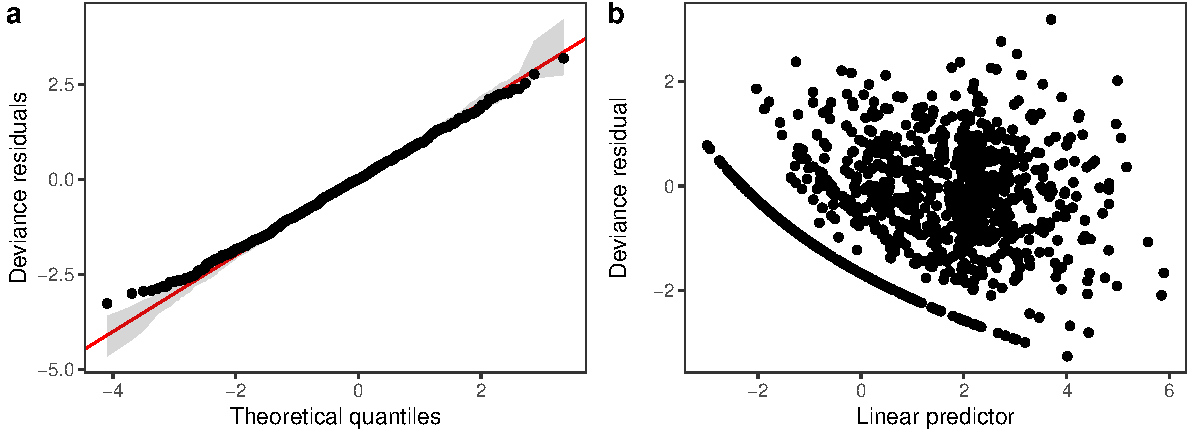
\includegraphics{../figures/zoo_comm_diag-1.pdf}
\caption{\label{fig:zoo_comm_diag_plot} Diagnostic plots for model
\emph{I} fitted to zooplankton community data in Lake Mendota. a)
QQ-plot of residuals (black). Red line indicates the 1-1 line and grey
bands correspond to the expected 95\% CI for the QQ plot, assuming the
distribution is correct. b) Deviance residuals versus fitted values (on
the link scale).}
\end{figure}

Differences between models \emph{S} (shared smoothness between taxa) and
\emph{I} (different smoothness for each taxa) seem to be driven by the
low seasonality of \emph{L. siciloides} relative to the other species,
and how this is captured by the more flexible model \emph{I} (Figure
\ref{fig:zoo_comp}). Still, both models show very similar fits to the
training data. This implies that the added complexity of different
penalties for each species (model \emph{I}) is unnessecary here, which
is consistent with the fact that model \emph{S} has a lower AIC (4667)
than model \emph{I} (4677), and that model \emph{S} is somewhat better
at predicting out-of-sample fits for all taxa than model \emph{I} (Table
\ref{tab:zoo_comm_outofsample_kable}). Both models show significant
predictive improvement compared to the intercept-only model for all
species except \emph{K. cochlearis} (Table
\ref{tab:zoo_comm_outofsample_kable}). This may be driven by changing
timing of the spring bloom for this species between training and
out-of-sample years (Figure \ref{fig:zoo_comp}).

\begin{figure}
\centering
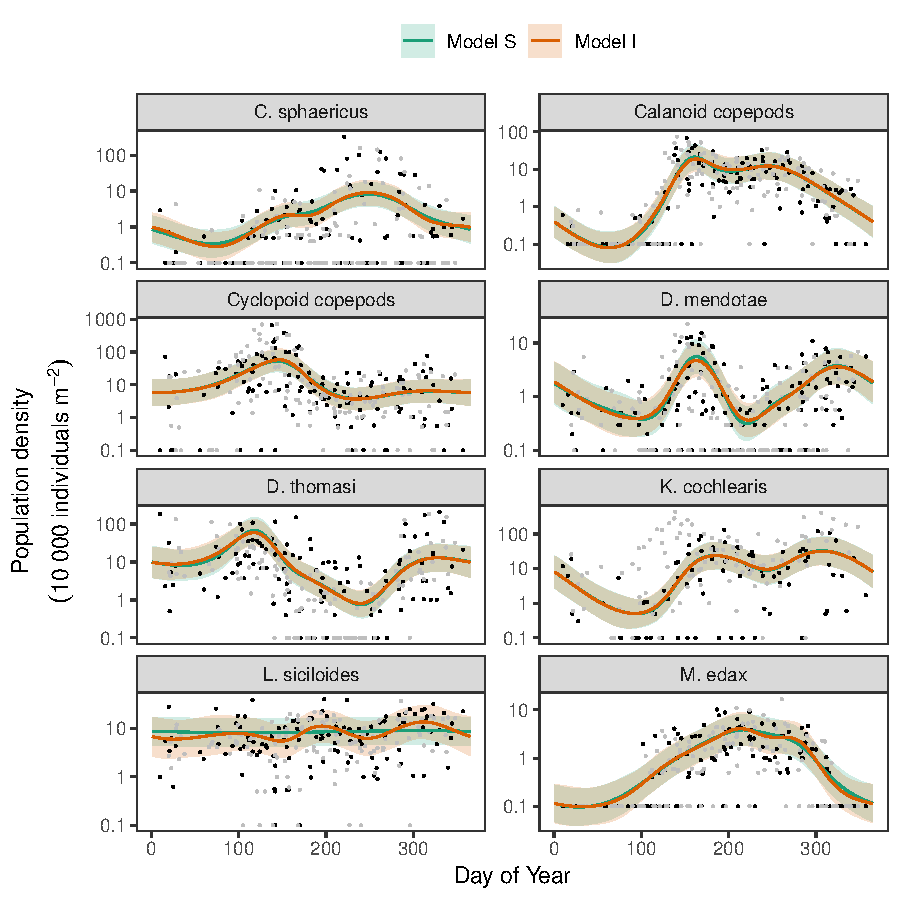
\includegraphics{../figures/zoo_comm_plot-1.pdf}
\caption{\label{fig:zoo_comp}Species-specific seasonal dynamics for the
eight zooplankon species tracked in Lake Mendota. Black points indicate
individual plankton observations in the training data, and grey points
are observations in held-out years used for model validation. Lines
indicate predicted average values for model \emph{S} (black) and model
\emph{I} (red). Ribbons indicate \(\pm\) 2 standard errors around the
mean.}
\end{figure}

\begin{table}[t]

\caption{\label{tab:zoo_comm_outofsample_kable}Out-of-sample predictive ability for model \textit{S} and \textit{I} applied to the zooplankton community dataset. Deviance values represent the total deviance of model predictions from observations for out-of-sample data. 'Intercept only' results are for a null model with only taxon-level random effect intercepts included.}
\centering
\begin{tabular}{llll}
\toprule
\multicolumn{1}{c}{ } & \multicolumn{3}{c}{Total deviance of out-of-sample data} \\
\cmidrule(l{2pt}r{2pt}){2-4}
taxon & Intercept only & Model S & Model I\\
\midrule
\em{C. sphaericus} & 715 & 482 & 495\\
Calanoid copepods & 346 & 220 & 223\\
Cyclopoid copepods & 569 & 381 & 386\\
\em{D. mendotae} & 353 & 264 & 268\\
\em{D. thomasi} & 486 & 333 & 337\\
\addlinespace
\em{K. cochlearis} & 486 & 2260 & 2340\\
\em{L. siciloides} & 132 & 116 & 126\\
\em{M. edax} & 270 & 138 & 139\\
\bottomrule
\end{tabular}
\end{table}

Next, we look at how to fit inter-lake variability in dynamics for just
\emph{Daphnia mendotae}. Here, we will compare models \emph{G},
\emph{GS}, and \emph{GI} to determine if a single global function is
appropriate for all four lakes, or if we can more effectively model
variation between lakes with a shared smoother and lake-specific
smoothers.

\subsubsection{\texorpdfstring{Model
\emph{G}:}{Model G:}}\label{model-g}

\begin{Shaded}
\begin{Highlighting}[]
\NormalTok{zoo_daph_modG <-}\StringTok{ }\KeywordTok{gam}\NormalTok{(density_adj }\OperatorTok{~}\StringTok{ }\KeywordTok{s}\NormalTok{(day, }\DataTypeTok{bs=}\StringTok{"cc"}\NormalTok{, }\DataTypeTok{k=}\DecValTok{10}\NormalTok{)}\OperatorTok{+}
\StringTok{                       }\KeywordTok{s}\NormalTok{(lake, }\DataTypeTok{bs=}\StringTok{"re"}\NormalTok{) }\OperatorTok{+}\StringTok{ }
\StringTok{                       }\KeywordTok{s}\NormalTok{(lake, year_f,}\DataTypeTok{bs=}\StringTok{"re"}\NormalTok{),}
                     \DataTypeTok{data=}\NormalTok{daphnia_train,}
                     \DataTypeTok{knots=}\KeywordTok{list}\NormalTok{(}\DataTypeTok{day =}\KeywordTok{c}\NormalTok{(}\DecValTok{0}\NormalTok{, }\DecValTok{365}\NormalTok{)),}
                     \DataTypeTok{family=}\KeywordTok{Gamma}\NormalTok{(}\DataTypeTok{link =}\StringTok{"log"}\NormalTok{),}
                     \DataTypeTok{method=}\StringTok{"REML"}\NormalTok{,}
                     \DataTypeTok{drop.unused.levels =} \OtherTok{FALSE}\NormalTok{)}
\end{Highlighting}
\end{Shaded}

\subsubsection{\texorpdfstring{Model
\emph{GS}:}{Model GS:}}\label{model-gs}

\begin{Shaded}
\begin{Highlighting}[]
\NormalTok{zoo_daph_modGS <-}
\StringTok{  }\KeywordTok{gam}\NormalTok{(density_adj }\OperatorTok{~}\StringTok{ }\KeywordTok{s}\NormalTok{(day, }\DataTypeTok{bs=}\StringTok{"cc"}\NormalTok{, }\DataTypeTok{k=}\DecValTok{10}\NormalTok{) }\OperatorTok{+}\StringTok{ }
\StringTok{        }\KeywordTok{s}\NormalTok{(day, lake, }\DataTypeTok{k=}\DecValTok{10}\NormalTok{, }\DataTypeTok{bs=}\StringTok{"fs"}\NormalTok{, }\DataTypeTok{xt=}\KeywordTok{list}\NormalTok{(}\DataTypeTok{bs=}\StringTok{"cc"}\NormalTok{)) }\OperatorTok{+}\StringTok{ }
\StringTok{        }\KeywordTok{s}\NormalTok{(lake, year_f,}\DataTypeTok{bs=}\StringTok{"re"}\NormalTok{),}
      \DataTypeTok{data=}\NormalTok{daphnia_train, }
      \DataTypeTok{knots=}\KeywordTok{list}\NormalTok{(}\DataTypeTok{day=}\KeywordTok{c}\NormalTok{(}\DecValTok{0}\NormalTok{, }\DecValTok{365}\NormalTok{)), }
      \DataTypeTok{family=}\KeywordTok{Gamma}\NormalTok{(}\DataTypeTok{link =}\StringTok{"log"}\NormalTok{),}
      \DataTypeTok{drop.unused.levels =} \OtherTok{FALSE}\NormalTok{,}
      \DataTypeTok{method=}\StringTok{"REML"}\NormalTok{)}
\end{Highlighting}
\end{Shaded}

\subsubsection{\texorpdfstring{Model
\emph{GI}:}{Model GI:}}\label{model-gi}

\begin{Shaded}
\begin{Highlighting}[]
\NormalTok{zoo_daph_modGI <-}\StringTok{ }\KeywordTok{gam}\NormalTok{(density_adj}\OperatorTok{~}\KeywordTok{s}\NormalTok{(day, }\DataTypeTok{bs=}\StringTok{"cc"}\NormalTok{, }\DataTypeTok{k=}\DecValTok{10}\NormalTok{) }\OperatorTok{+}
\StringTok{                             }\KeywordTok{s}\NormalTok{(day, }\DataTypeTok{by=}\NormalTok{lake, }\DataTypeTok{k=}\DecValTok{10}\NormalTok{, }\DataTypeTok{bs=}\StringTok{"cc"}\NormalTok{)}\OperatorTok{+}
\StringTok{                             }\KeywordTok{s}\NormalTok{(lake, }\DataTypeTok{bs=}\StringTok{"re"}\NormalTok{) }\OperatorTok{+}\StringTok{ }
\StringTok{                             }\KeywordTok{s}\NormalTok{(lake, year_f,}\DataTypeTok{bs=}\StringTok{"re"}\NormalTok{),}
                     \DataTypeTok{data=}\NormalTok{daphnia_train,}
                     \DataTypeTok{knots=}\KeywordTok{list}\NormalTok{(}\DataTypeTok{day =}\KeywordTok{c}\NormalTok{(}\DecValTok{0}\NormalTok{, }\DecValTok{365}\NormalTok{)),}
                     \DataTypeTok{family=}\KeywordTok{Gamma}\NormalTok{(}\DataTypeTok{link =}\StringTok{"log"}\NormalTok{),}
                     \DataTypeTok{method=}\StringTok{"REML"}\NormalTok{,}
                     \DataTypeTok{drop.unused.levels =} \OtherTok{FALSE}\NormalTok{)}
\end{Highlighting}
\end{Shaded}

Diagnostic plots from \texttt{gam.check} indicate that there are no
substantial patterns comparing residuals to fitted values (not shown),
and QQ-plots are similiar to the those from the zooplankton community
models; the residuals for all three models closely correspond to the
expected (Gamma) distribution, except at small values, where the
observed residuals are generally larger than expected (Fig.
\ref{fig:zoo_daph_diag_plot}). As with the community data, this is
likely an artifact of the assumption we made of assigning zero
observations a value of 1000 (the lowest possible value), imposing an
artifical lower bound on the observed counts. There was also some
evidence that the largest observed values were smaller than expected
given the theoretical distribution , but these fell within the 95\% CI
for expected deviations from the 1-1 line (Fig.
\ref{fig:zoo_daph_diag_plot}).

\begin{figure}
\centering
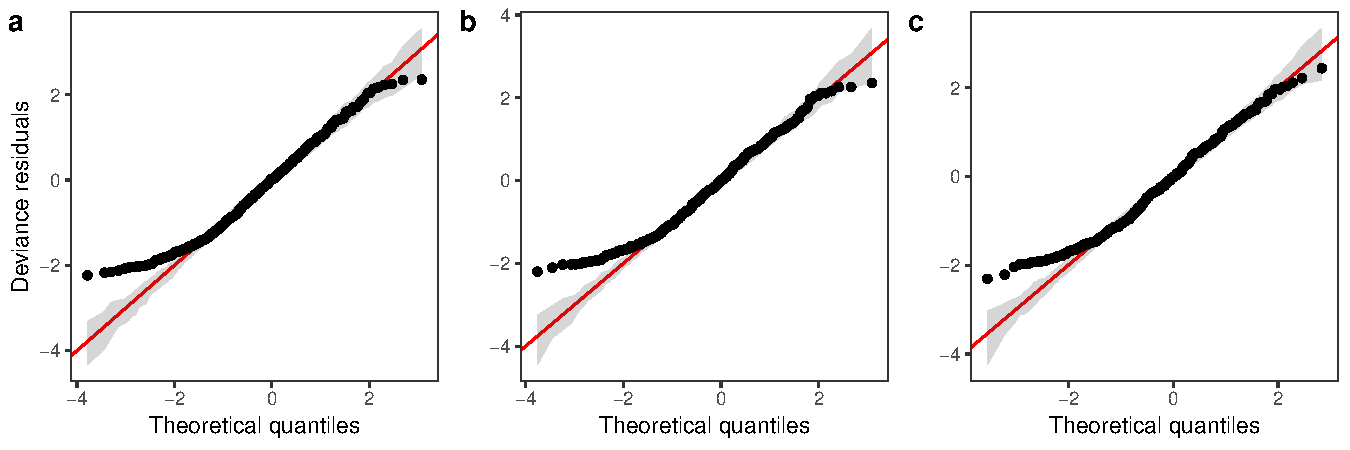
\includegraphics{../figures/zoo_daph_diag-1.pdf}
\caption{\label{fig:zoo_daph_diag_plot} QQ-plots for model \emph{G} (a)
, \emph{GS} (b), and \emph{GI} (c) fitted to Daphnia data across the
four lakes. Red line indicates the 1-1 line, black points are observed
model residuals, and grey bands correspond to the expected 95\% CI for
the QQ plot, assuming the distribution is correct.}
\end{figure}

The AIC values indicate that both model \emph{GS} (1093.71) and
\emph{GI} (1085.7) are better fits than model \emph{G} (1097.62), but
models \emph{GI} fits somewhat better than model \emph{GS}.\footnote{When
  comparing models via AIC, we use the standard rule of thumb from
  Burnham \& Anderson (1998), where models that differ by 2 units or
  less from the lowest AIC model have substantial support, and those
  differing by more than 4 units having less support.} There does not
seem to be a large amount of inter-lake variability (the effective
degrees of freedom per lake are low in models \emph{GS} \& \emph{GI}).
Plots for all three models (Figure \ref{fig:daph_smooth}) show that
Mendota, Monona, and Kegonsa lakes are very close to the average and to
one another for both models, but Waubesa shows evidence of a more
pronounced spring bloom and lower winter abundances.

\begin{figure}
\centering
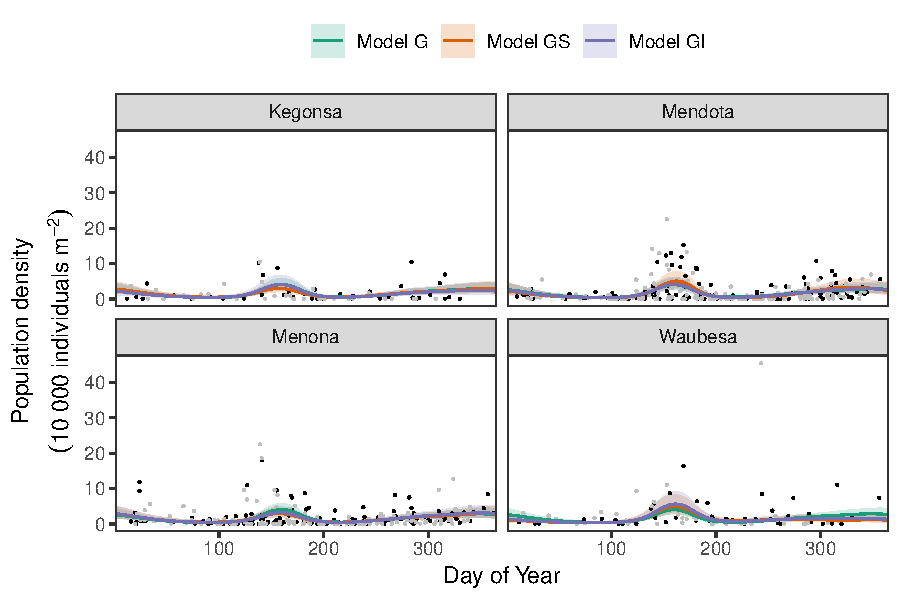
\includegraphics{../figures/zoo_daph_plot-1.pdf}
\caption{\label{fig:daph_smooth}Raw data (points) and fitted models
(lines) for \textit{D. mendota} data. Black points indicate individual
plankton observations in the training data, and grey points are
observations in held-out years used for model validation. Green line:
model \emph{G} (no inter-lake variation in dynamics); orange line: model
\emph{GS} (interlake variation with similar smoothness); purple line:
model \emph{GI} (varying smoothness among lakes). Shaded bands are drawn
at \(\pm\) 2 standard errors around each model.}
\end{figure}

Model \emph{GI} is able to predict as well or better than model \emph{G}
or \emph{GS} for all lakes (Table \ref{tab:zoo_daph_outofsample_kable}),
indicating that allowing for inter-lake variation in seasonal dynamics
improved model prediction. All three models predicted dynamics in Lake
Mendota and Lake Menona significantly better than the intercept-only
model (Table \ref{tab:zoo_daph_outofsample_kable}). None of the models
did well in terms of predicting Lake Waubesa dynamics out-of-sample
compared to a simple model with only a lake-specific intercept and no
intra-annual variability, but this was due to the influence of a single
very large outlier in the out-of-sample data (Figure
\ref{fig:daph_smooth} bottom right). However, baring a more detailed
investigation into the cause of this large value, we cannot arbitrarily
exclude this outlier from the goodness-of-fit analysis; it may be due
either to measurement error or a true high late-season \emph{Daphnia}
density that our model was not able to predict.

\begin{table}[t]

\caption{\label{tab:zoo_daph_outofsample_kable}Out-of-sample predictive ability for model \textit{G}, \textit{GS}, and \textit{GI} applied to the \textit{D. mendotae} dataset. Deviance values represent the total deviance of model predictions from observations for out-of-sample data. 'Intercept only' results are for a null model with only lake-level random effect intercepts included.}
\centering
\begin{tabular}{lllll}
\toprule
\multicolumn{1}{c}{ } & \multicolumn{4}{c}{Total deviance of out-of-sample data} \\
\cmidrule(l{2pt}r{2pt}){2-5}
Lake & Intercept only & Model G & Model GS & Model GI\\
\midrule
Kegonsa & 96 & 92 & 89 & 86\\
Mendota & 352 & 258 & 257 & 257\\
Menona & 348 & 300 & 294 & 290\\
Waubesa & 113 & 176 & 164 & 157\\
\bottomrule
\end{tabular}
\end{table}

\FloatBarrier

\section{V: Computational and statistical issues when fitting
HGAMs}\label{v-computational-and-statistical-issues-when-fitting-hgams}

Which of the five model formulations (figure \ref{fig:models}) should
you choose for a given data set? There are two major trade-offs to
consider. The first is the bias-variance trade-off: more complex models
can account for more fluctuations in the data, but also tend to give
more variable predictions, and can overfit. The second trade-off is
model complexity versus computational cost: more complex models can
include more potential sources of variation and give more information
about a given data set, but will generally take more time and
computational resources to fit and debug. We discuss both of these
trade-offs in this section. We also discuss how to extend the HGAM
framework to fit more complex models.

\subsection{Bias-variance trade-offs}\label{bias-variance-trade-offs}

The bias-variance trade-off is a fundamental concept in statistics. When
trying to estimate any relationship (in the case of GAMs, a smooth
relationship between predictors and data) bias measures how far, on
average, an estimate is from the true value. The variance of an
estimator corresponds to how much that estimator would fluctuate if
applied to multiple different samples of the same size taken from the
same population. These two properties tend to be traded off when fitting
models. For instance, rather than estimating a population mean from
data, we could simply use a predetermined fixed value regardless of the
observed data\footnote{While this example may seem contrived, this is
  exactly what happens when we assume a given regression coefficient is
  equal to zero (and thus exclude it from a model).}. This estimate
would have no variance (as it is always the same regardless of what the
data look like) but would have high bias unless the true population mean
happened to equal the fixed value we chose. Penalization is useful
because using a penalty term slightly increases model bias, but can
substantially decrease variance (Efron \& Morris, 1977).

In GAMs, the bias-variance trade-off is managed by the terms of the
penalty matrix, and equivalently random effect variances in HGLMs.
Larger penalties correspond to lower variance, as the estimated function
is unable to wiggle a great deal, but also correspond to higher bias
unless the true function is close to the null space for a given smoother
(e.g., a straight line for thin plate splines with 2nd derivative
penalties, or zero for a random effect). The computational machinery
used by \textbf{mgcv} to fit smooth terms is designed to find penalty
terms that best trade-off bias for variance to find a smoother that can
effectively predict new data.

The bias-variance trade-off comes into play with HGAMs when choosing
whether to fit separate penalties for each group level or assign a
common penalty for all group levels (i.e., deciding between models
\emph{GS} \& \emph{GI} or models \emph{S} \& \emph{I}). If the
functional relationships we are trying to estimate for different group
levels actually vary in how wiggly they are, setting the penalty for all
group-level smoothers equal (models \emph{GS} \& \emph{S}) will either
lead to overly variable estimates for the least variable group levels,
over-smoothed (biased) estimates for the most wiggly terms, or a mixture
of these two, depending on the fitting criteria.

We developed a simple numerical experiment to determine whether
\textbf{mgcv}'s fitting criteria tend to set estimated smoothness
penalties high or low in the presence of among-group variability in
smoothness when fitting model \emph{GS} or \emph{S} HGAMs. We simulated
data from four different groups, with all groups having the same levels
of the covariate \(x\), equally spaced across the range from 0 to
\(2\pi\). For each group, the true function relating \(x\) to the
response, \(y\), was a cosine wave, but the frequency varied from 0.5
(equal to half a cycle across the range of \(x\)) to 4 (corresponding to
4 full cycles across the range). As all four sin waves spanned the whole
range from -1 to +1 across the range of x, and as they were all integer
or half-integer frequencies, the signal for all groups had the same
variance across the range of \(x\), approximately equal to 0.5.
Therefore, the true function for all groups had the same strength of
signal; all that varied between groups was how rapidly the signal
fluctuated. We added normally distributed error to all \(y\)-values,
with three different noise levels, given by standard deviations of
0.5,1, and 2. These correspond to signal-to-noise ratios (i.e.~variance
of the cosine curve divided by variance of the noise) of 2, 0.5, and
0.125. For each noise level, we created 25 replicate data sets, to
illustrate the amount of simulation-to-simulation variation in model
fit. We then fit both model \emph{S} (where all curves were assumed to
be equally smooth) and model \emph{I} (with varying smoothness) to each
replicate for each noise level, using REML criteria to estimate
penalties.

A sample of the fits for each group for three of the replicates for each
model are shown in Fig. \ref{fig:var_pen}a, with model \emph{S} in red
and model \emph{I} in blue. Fig. \ref{fig:var_pen}b illustrates how well
each model fared across the range of replicates at accurately estimating
the true smoothness of the highest frequency terms as measured by the
squared second derivative of the smooth fit versus that of the true
function, with the distance to the black one-to-one line indicating the
degree to which the estimated function for each group over- or
under-estimated the smoothness of the true signal. In general, under low
noise conditions (Fig \ref{fig:var_pen}, signal-to-noise ratio of 2),
model \emph{S} tendeded to overfit the smoothest, lowest-frequency,
groups, while accurately fitting the highest frequency groups. Under
moderate signal-to-noise ratios, model \emph{S} tended to over-penalize
high-frequency groups and under-penalize low frequency groups, and in
the lowest signal-to-noise ratio tested (0.125), model \emph{S} tended
to penalize all groups towards very smooth functions (Fig.
\ref{fig:var_pen}b). Curves estimated by model \emph{I}, on the other
hand, tended to accurately capture the true wiggliness of the function
across the whole range of frequencies and noises, except for the
lowest-frequency groups, and the highest frequency groups it the
presence of high noise; in both cases, model \emph{I} tended to
over-smooth (.Fig. \ref{fig:var_pen}b).

This implies that assuming equal smoothness will result in
underestimating the true smoothness of low-variability terms in cases of
high signal-to-noise, and overestimating the true smoothness of
high-frequency terms in low signal-to-noise data sets. If this is a
potential issue, we recommend fitting both models \emph{S} and \emph{I}
and using standard model evaluation criteria (e.g., AIC) or
out-of-sample predictive accuracy (as in Section IV) to determine if
there is evidence for among-group variability in smoothness. However, it
may be the case that there are too few data points per group to estimate
separate smoothness levels, in which case model \emph{GS} or model
\emph{S} may still be the better option even in the face of varying
smoothness.

The ideal case would be to assume that among-group penalties follow
their own distribution (estimated from the data), to allow variation in
smoothness while still getting the benefit of pooling information on
smoothness between groups. This is currently not implemented in
\textbf{mgcv}. It is possible to set up this type of varying penalty
model in flexible Bayesian modelling software such as \emph{Stan} (see
below for a discussion of how to fit HGAMs using these tools), where
inter-group variation in smoothing penalties could be modelled with a
hierarchical prior. However, to the best of our knowledge, how to fit
this type of model has not been well studied in either the Bayesian or
frequentist literature.

\begin{figure}
\centering
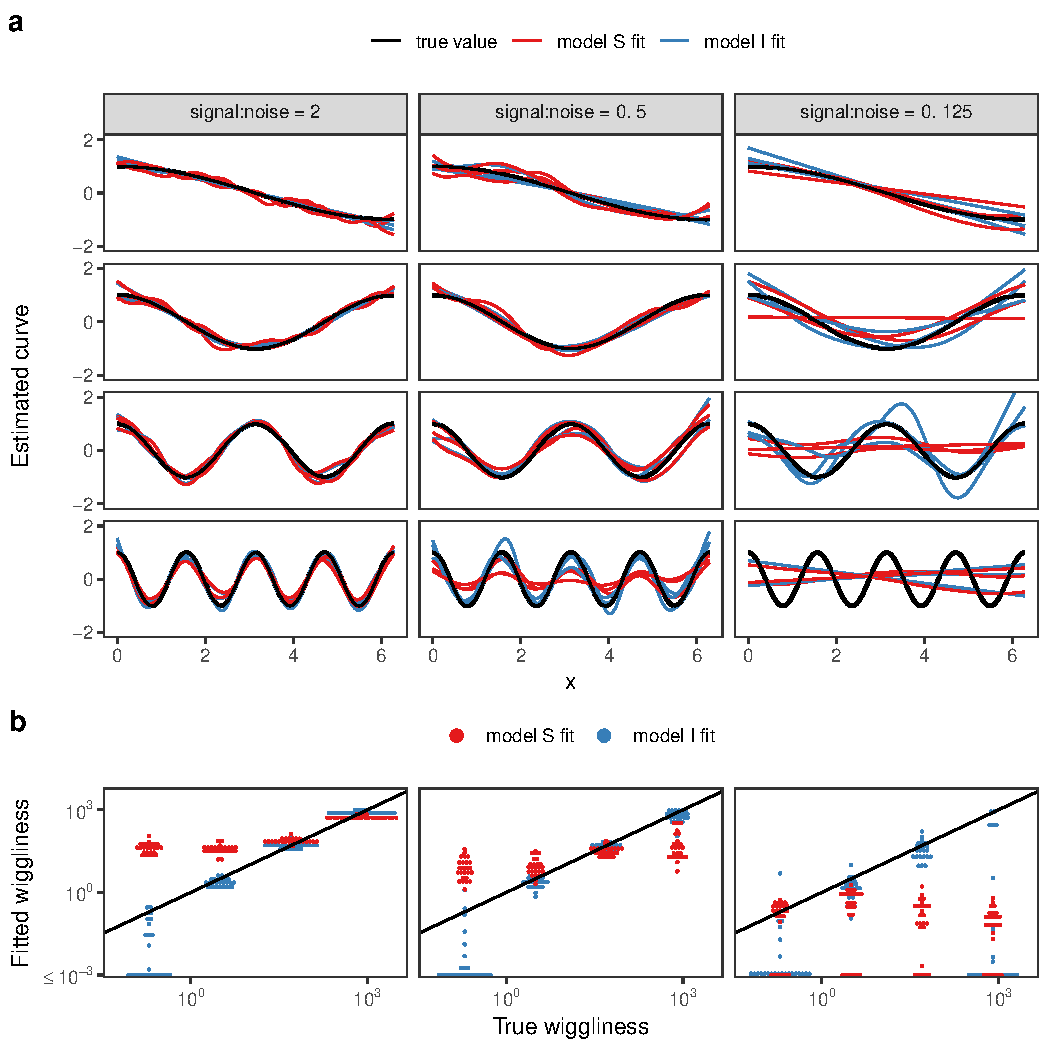
\includegraphics{../figures/single_smooth_bias_plot-1.pdf}
\caption{\label{fig:var_pen} a) Illustration of bias that can arise from
assuming equal smoothness for all group levels (model \emph{S}, red
lines) versus allowing for intergroup variation in smoothness (model
\emph{I}, blue lines) across a range of signal-to-noise ratios, holding
the group-level signals constant. The true function for each group level
is shown in black. b) Distribution of wiggliness (as measured by the
integral of the squared 2nd derivative) of the estimated function for
each replicate for each group level for model \emph{S} (red) and model
\emph{I} (blue), versus the true wiggliness of the function for that
grouping level, with the black line indicating the one-to-one line.
Points below (above) the black line indicate that a given model
estimated the curve as less (more) wiggly than the true curve used to
generate the data. Estimated wiggliness less than \(10^{-3}\) was
truncated for visual clarity, as \textbf{mgcv} estimated effectively
straight lines for several groups, corresponding to a wiggliness of 0,
which would not appear on a log-scaled plot.}
\end{figure}

It may seem there is also a bias-variance trade-off between choosing to
use a single global smoother (model \emph{G}) or a global smoother plus
group-level terms (models \emph{GS} and \emph{GI}). In model \emph{G},
all the data is used to estimate a single smooth term, and thus should
have lower variance than models \emph{GS} and \emph{GI}, but higher bias
for any given group in the presence of inter-group functional
variability. However, in practice, this trade-off will be handled via
penalization; if there are no average differences between functional
responses, \textbf{mgcv} will penalize the group-specific functions
toward zero, and thus toward the global model. The choice between using
model \emph{G} versus models \emph{GS} and \emph{GI} should generally be
driven by computational costs. Model \emph{G} is typically much faster
to fit than models \emph{GS} and \emph{GI}, even in the absence of
among-group differences. If there is no need to estimate inter-group
variability, model \emph{G} will typically be more efficient.

A similar issue exists when choosing between models \emph{GS} and
\emph{GI} and models \emph{S} and \emph{I}. If all group levels have
very different functional shapes, the global term will get penalized
toward zero in models \emph{GS} and \emph{GI}, so they will reduce to
models \emph{S} and \emph{I}. The choice to include a global term should
be made based on scientific considerations (is the global term of
interest?) and computational considerations.

\subsection{Complexity-computation
trade-offs}\label{complexity-computation-trade-offs}

The more flexible a model is, the larger an effective parameter space
any fitting software has to search. It can be surprisingly easy to use
massive computational resources trying to fit models to even small
datasets. While we typically want to select models based on their fit
and our inferential goals, computing resources can often act as an
effective upper bound on model complexity. For a given data set,
assuming a fixed family and link function, the time taken to estimate an
HGAM will depend (roughly) on four factors: \emph{(i)} the number of
coefficients to be estimated (and thus the number of basis functions
chosen), \emph{(ii)} the number of smoothing parameters to be estimated,
\emph{(iii)} whether the model needs to estimate both a global smoother
and groupwise smoothers, and \emph{(iv)} the algorithm and fitting
criteria used to estimate parameters.

The most straightforward factor that will affect the amount of
computational resources is the number of parameters in the model. Adding
group-level smoothers (moving from model \emph{G} to the other models)
means that there will be more regression parameters to estimate. For a
dataset with \(g\) different groups and \(n\) data points, fitting a
model with just a global smoother, \texttt{y\textasciitilde{}s(x,k=k)}
will require \(k\) coefficients, and takes \(\mathcal{O}(nk^2)\)
operations to evaluate. Fitting the same data using a group-level
smoother (model \emph{S},
\texttt{y\textasciitilde{}s(x,fac,bs="fs",k=k)}) will require
\(\mathcal{O}(nk^2g^2)\) operations to evaluate. In effect, adding a
group-level smoother will increase computational cost by an order of the
number of groups squared. The effect of this is visible in the examples
we fit in section III. Table \ref{tab:comp_time_kable} compares the
relative time it takes to compute model \emph{G} versus the other
models.

One way to deal with this issue would be to reduce the number of basis
functions used when fitting group-level smoothers when the number of
groups is large, limiting the flexibility of the model. It can also make
sense to use more computationally-efficient basis functions when fitting
large data sets, such as P-splines (Wood, 2017b) or cubic splines. Thin
plate splines entail greater computational costs (Wood, 2017a).

Including a global smoother (models \emph{GS} and \emph{GI} compared to
models \emph{S} and \emph{I}) will not generally substantially affect
the number of coefficients that need to be estimated (Table
\ref{tab:comp_time_kable}). Adding a global term will add at most
\texttt{k} extra terms. It can be substantially less than that, as
\textbf{mgcv} drops basis functions from co-linear smoothers to ensure
that the model matrix is full rank.

Adding additional smoothing parameters (moving from model \emph{GS} to
\emph{GI}, or moving from model \emph{S} to \emph{I}) is more costly
than increasing the number of coefficients to estimate, as estimating
smoothing parameters is computationally intensive (Wood, 2011). This
means that models \emph{GS} and \emph{S} will generally be substantially
faster than \emph{GI} and \emph{I} when the number of groups is large,
as models \emph{GI} and \emph{I} fit a separate set of penalties for
each group level. The effect of this is visible in comparing the time it
takes to fit model \emph{GS} to model \emph{GI} (which has a smoother
for each group) or models \emph{S} and \emph{I} for the example data
(Table \ref{tab:comp_time_kable}). Note that this will not hold in all
cases. For instance, model \emph{I} takes less time to fit the bird
movement data than model \emph{S} does (Table
\ref{tab:comp_time_kable}B).

\begin{table}[t]

\caption{\label{tab:comp_time_kable}Relative computational time and model complexity for different HGAM formulations of the two example data sets from section III. All times are scaled relative to the length of time model *G* takes to fit to that data set. The number of coefficients measures the total number of model parameters (including intercepts). The number of smoothers is the total number of unique penalty values estimated by the model.}
\centering
\begin{tabular}{lrrr}
\toprule
\multicolumn{1}{c}{ } & \multicolumn{1}{c}{ } & \multicolumn{2}{c}{\# of terms} \\
\cmidrule(l{2pt}r{2pt}){3-4}
model & relative time & coefficients & penalties\\
\midrule
\addlinespace[0.3em]
\multicolumn{4}{l}{\textbf{A. CO2 data}}\\
\hspace{1em}G & 1 & 17 & 2\\
\hspace{1em}GS & 14 & 65 & 14\\
\hspace{1em}GI & 7 & 65 & 3\\
\hspace{1em}S & 18 & 61 & 13\\
\hspace{1em}I & 6 & 61 & 3\\
\addlinespace[0.3em]
\multicolumn{4}{l}{\textbf{B. bird movement data}}\\
\hspace{1em}G & 1 & 90 & 2\\
\hspace{1em}GS & 320 & 624 & 14\\
\hspace{1em}GI & 150 & 540 & 5\\
\hspace{1em}S & 65 & 535 & 12\\
\hspace{1em}I & 120 & 541 & 3\\
\bottomrule
\end{tabular}
\end{table}

\subsection{\texorpdfstring{Alternative formulations: \texttt{bam()},
\texttt{gamm()}, and
\texttt{gamm4()}}{Alternative formulations: bam(), gamm(), and gamm4()}}\label{alternative-formulations-bam-gamm-and-gamm4}

When fitting models with large numbers of groups, it is often possible
to speed up computation substantially by using one of the alternative
fitting routines available through \textbf{mgcv}.

The first option is the function \texttt{bam()}, this requires the least
changes to existing code written using the \texttt{gam()} function.
\texttt{bam()} is designed to improve performance when fitting large
data sets via two mechanisms. First, it saves on memory needed to
compute a given model by using a random subset of the data to calculate
the basis functions. It then blocks the data and updates model fit
within each block (Wood, Goude \& Shaw, 2015). While this is primarily
designed to reduce memory usage, it can also substantially reduce
computation time. Second, when using \texttt{bam()}'s default fREML
(``Fast REML'') method, you can use the \texttt{discrete=TRUE} option:
this first bins continuous covariates into a smaller number of discrete
values before estimating the model, substantially reducing the amount of
computation needed (Wood et al. (2017); see \texttt{?mgcv::bam} for more
details). Setting up the five model types (figure \ref{fig:models}) in
\texttt{bam()} uses the same code as we have previously covered; the
only difference is that you use the \texttt{bam()} instead of
\texttt{gam()} function, and have the additional option of discretizing
your covariates.

\texttt{bam()} has a larger computational overhead than \texttt{gam()},
so for small numbers of groups, it can be slower than \texttt{gam()}
(Figure~\ref{fig:alt_timing}). As the number of groups increases,
computational time for \texttt{bam()} increases more slowly than for
\texttt{gam()}; in our simulation tests, when the number of groups is
greater than 16, \texttt{bam()} can be upward of an order of magnitude
faster (Figure \ref{fig:alt_timing}). Note that \texttt{bam()} can be
somewhat less computationally stable when estimating these models (i.e.,
less likely to converge).

The second option is to fit models using one of two dedicated mixed
effect model estimation packages, \textbf{nlme} and \textbf{lme4}. The
\textbf{mgcv} package includes the function \texttt{gamm()}, which uses
the \textbf{nlme} package to estimate the GAM, automatically handling
the transformation of smooth terms into random effects (and back into
basis function representations for plotting and other statistical
analyses). The \texttt{gamm4()} function, in the separate \textbf{gamm4}
package, uses \textbf{lme4} in a similar way. Using \texttt{gamm()} or
\texttt{gamm4()} to fit models rather than \texttt{gam()} can
substantially speed up computation when the number of groups is large,
as both \textbf{nlme} and \textbf{lme4} take advantage of the sparse
structure of the random effects, where most basis functions will be zero
for most groups (i.e., any group-specific basis function will only take
a non-zero value for observations in that group level). As with
\texttt{bam()}, \texttt{gamm()} and \texttt{gamm4()} are generally
slower than \texttt{gam()} for fitting HGAMs when the number of group
levels is small (in our simulations, \textless{}8 group levels), however
they do show substantial speed improvements even with a moderate number
of groups, and were as fast as or faster to calculate than
\texttt{bam()} for all numbers of grouping levels we tested (Figure
\ref{fig:alt_timing})\footnote{It is also possible to speed up both
  \texttt{gam()} and \texttt{bam()} by using multiple processors in
  parallel, whereas this is not currently possible for \texttt{gamm()}
  and \texttt{gamm4()}. For large numbers of grouping levels, this
  should speed up computation as well, at the cost of using more memory.
  However, computation time will likely not decline linearly with the
  number of cores used, since not all model fitting sets are
  parallelizable, and performance of cores can vary. As parallel
  processing can be complicated and dependent on the type of computer
  you are using to configure, we do not go into how to use these methods
  here. The help file \texttt{?mgcv::mgcv.parallel} explains how to use
  parallel computations for \texttt{gam()} and \texttt{bam()} in detail.}.

\begin{figure}
\centering
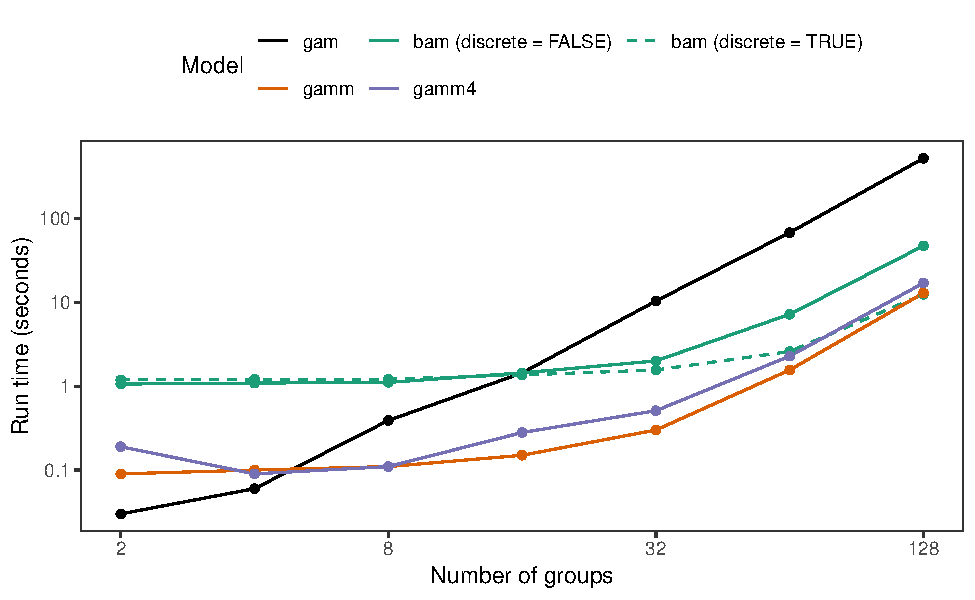
\includegraphics{../figures/alt_model_timing_plot-1.pdf}
\caption{\label{fig:alt_timing}Elapsed time to estimate the same model
using each of the four approaches. Each data set was generated with 20
observations per group using a unimodal global function and random
group-specific functions consisting of an intercept, a quadratic term,
and logistic trend for each group. Observation error was normally
distributed. Models were fit using model 2:
\texttt{y~s(x, k=10, bs="cp") + s(x,fac, k=10, bs="fs", xt=list(bs="cp"), m=1)}.
All models were run on a single core.}
\end{figure}

Both \texttt{gamm()} and \texttt{gamm4()} require a few changes to model
code. First, there are a few limitations on how you are able to specify
the different model types (figure \ref{fig:models}) in both frameworks.
Factor-smoother interaction (\texttt{bs="fs"}) basis setup works in both
\texttt{gamm()} and \texttt{gamm4()}. However, as the \textbf{nlme}
package does not support crossed random effects, it is not possible to
have two factor-smoother interaction terms for the same grouping
variable in \texttt{gamm()} models (e.g.,
\texttt{y\textasciitilde{}s(x1,\ grp,\ bs="fs")+s(x2,\ grp,\ bs="fs")}.
These type of crossed random effects are allowed in \textbf{gamm4}. The
use of \texttt{te()} terms are not possible in \textbf{gamm4}, due to
issues with how random effects are specified in the \textbf{lme4}
package, making it impossible to code models where multiple penalties
apply to a single basis function. Instead, for multidimensional
group-level smoothers, the alternate function \texttt{t2()} needs to be
used to generate these terms, as it creates tensor products with only a
single penalty for each basis function (see \texttt{?mgcv::t2} for
details on these smoothers, and Wood, Scheipl \& Faraway (2013) for the
theoretical basis behind this type of tensor product). For instance,
model \emph{GS} for the bird movement data we discussed in section III
would need to be coded as:

\begin{verbatim}
bird_modS_gamm4 <-
  gamm4(count ~ t2(week, latitude, species, bs=c("cc", "tp", "re"),
                   k=c(10, 10, 6), m=2),
        data=bird_move, family="poisson")
\end{verbatim}

These packages also do not support the same range of families for the
dependent variable; \texttt{gamm()} only supports non-Gaussian families
by using a fitting method called penalized quasi-likelihood (PQL) that
is slower and not as numerically stable as the methods used in
\texttt{gam()}, \texttt{bam()}, and \texttt{gamm4()}. Non-Gaussian
families are well supported by \textbf{lme4} (and thus \textbf{gamm4}),
but can only fit them using marginal likelihood (ML) rather than REML,
so may tend to over-smooth relative to \texttt{gam()} using REML
estimation. Further, neither \texttt{gamm()} nor \texttt{gamm4()}
supports several of the extended families available through
\textbf{mgcv}, such as zero-inflated, negative binomial, or ordered
categorical and multinomial distributions.

\subsection{Estimation issues when fitting both global and groupwise
smoothers}\label{estimation-issues-when-fitting-both-global-and-groupwise-smoothers}

When fitting models with separate global and groupwise smoothers (models
\emph{GS} and \emph{GI}), one issue to be aware of is concurvity between
the global smoother and groupwise terms. Concurvity measures how well
one smooth term can be approximated by some combination of the other
smooth terms in the model (see \texttt{?mgcv::concurvity} for details).
For models \emph{GS} and \emph{GI}, the global term is entirely
concurved with the groupwise smoothers. This is because, in the absence
of the global smooth term, it would be possible to recreate that average
effect by shifting all the groupwise smoothers so they were centered
around the global mean. In practical terms, this has the consequence of
increasing uncertainty around the global mean relative to a model with
only a global smoother. In some cases, it can result in the estimated
global smoother being close to flat, even in simulated examples with a
known strong global effect. This concurvity issue may also increase the
time it takes to fit these models (for example, compare the time it
takes to fit models \emph{GI} and \emph{I} in Table
\ref{tab:comp_time_kable}). These models can still be estimated because
of penalty terms; all of the methods we have discussed for fitting model
\emph{GS} (factor-smoother terms or random effect tensor products)
automatically create a penalty for the null space of the group-level
terms, so that only the global term has its own unpenalized null space.
Both the REML and ML criteria work to balance penalties between nested
smooth terms (this is why nested random effects can be fitted). We have
observed that \textbf{mgcv} still occasionally finds solutions with
simulated data where the global term is over-smoothed.

To avoid this issue, we recommend both careful choice of basis and
setting model degrees of freedom so that groupwise terms are either
slightly less flexible than the global term or have a smaller null
space. In the examples in section III, we used smoothers with an
unpenalized null space (standard thin plate splines) for the global
smoother and ones with no null space for the groupwise terms\footnote{For
  model \emph{GS} both the factor-smoother, and tensor products of
  random effect (``re'') and other smooth terms do not have a penalized
  nullspace by construction (they are full rank), as noted above. For
  model \emph{GI} groupwise terms, we used basis types that had a
  penalty added to the nullspace, so called ``shrinkage'' methods:
  \texttt{bs="ts"}, \texttt{"cs"}, or \texttt{"ps"} have this property.}.
When using thin plate splines, it may also help to use splines with a
lower order of derivative penalized in the groupwise smoothers than the
global smoothers, as lower-order ``tp'' splines have fewer basis
functions in the null space. For example, we used \texttt{m=2}
(penalizing squared second derivatives) for the global smoother, and
\texttt{m=1} (penalizing squared first derivatives) for groupwise
smoothers in models \emph{GS} and \emph{GI}. Another option is to use a
lower number of basis functions (\texttt{k}) for groupwise relative to
global terms. This will reduce the maximum flexibility possible in the
groupwise terms. We do caution that these are just rules of thumb. In
cases where an accurately estimated global smoother is essential, we
recommend either fitting model \emph{G} or using specialized functional
regression software such as the \texttt{fosr} function in the
\emph{refund} package (Scheipl, Staicu \& Greven, 2014), which allows
the user to enforce constraints on the groupwise smoothers so that they
always sum to zero at any given point (avoiding the collinearity issue).
Also, see below for more information on functional regression.

\subsection{A brief foray into the land of
Bayes}\label{a-brief-foray-into-the-land-of-bayes}

As mentioned in section II, the penalty matrix can also be treated as
the inverse of a prior covariance matrix for model parameters
\(\boldsymbol{\beta}\). Intuitively, the basis functions and penalty we
use form a prior (in the informal sense) on how we'd like our model term
to behave. REML gives an empirical Bayes estimate of the smooth model
(Laird \& Ware, 1982), where terms in the null space of the smoother
have improper, flat priors (i.e., any value for these terms are
considered equally likely), any terms in the range space are treated as
having a multivariate normal distribution, and the penalty terms are
treated as having an improper flat prior (see Wood (2017a) Section 5.8
for more details on this connection). The large-sample approximation of
the posterior Bayesian covariance matrix (Wood, 2006b) for model
parameters can be extracted from any fitted \texttt{gam()} or
\texttt{bam()} model with \texttt{vcov(model)}. This can in turn be used
to generate samples from the posterior distribution of the model, as the
approximate Bayesian covariance matrix already incorporates the
uncertainty from having to estimate the covariance matrix into it (the
standard confidence intervals used in \textbf{mgcv} are in fact Bayesian
posterior credible intervals, which happen to have good frequentist
properties; Wood, 2006b; Marra \& Wood, 2012). Viewing our GAM as
Bayesian is a somewhat unavoidable consequence of the equivalence of
random effects and splines --- if we think that there is some true
smoother that we wish to estimate, we must take a Bayesian view of our
random effects (splines) as we do not think that the true smoother
changes each time we collect data (Wood, 2017a, Section 5.8).

This also means that HGAMs can be included as components in a more
complex fully Bayesian model. The \textbf{mgcv} package includes a
function \texttt{jagam()} that can take a specified model formula and
automatically convert it into code for the JAGS (or BUGS) Bayesian
statistical packages, which can be adapted by the user to their own
needs.

Similarly, the \textbf{brms} package (Bürkner, 2017), which can fit
complex statistical models using the Bayesian software \textbf{Stan}
(Carpenter et al., 2017) allows for the inclusion of \textbf{mgcv}-style
smooth terms as part of the model specification. The \textbf{brms}
package does not currently support \texttt{te()} tensor products, but
does support factor-smooth interactions and \texttt{t2()}-style tensor
products, which means all of the models fitted in this paper can be fit
by \textbf{brms}.

\subsection{Beyond HGAMs: functional
regression}\label{beyond-hgams-functional-regression}

The HGAMs we have discussed are actually a type of \emph{functional
regression}, which is an extension of standard regression models to
cases where the outcome variable \(y_i\) and/or the predictor variables
\(x_i\) for a given outcome are functions, rather than single variables
(Ramsay \& Silverman, 2005). HGAMs as we have described them are a form
of function-on-scalar regression (Ramsay \& Silverman, 2005; Reiss,
Huang \& Mennes, 2010), where we are trying to estimate a smooth
function that varies between grouping levels. Here the ``scalar'' refers
to the grouping level, and the function is the smooth term that varies
between levels; in contrast, a standard GAM is a type of
scalar-on-scalar regression, as the goal is to use a set of single
values (scalars) to estimate each (scalar) response.

We have deliberately focused our paper on these simpler classes of
functional regression model, and chosen to use the term HGAM rather than
functional regression, as we believe that this more clearly connects
these models to modelling approaches already familiar to ecologists.
Further, we consider the unit of analysis to still be individual
observations, as compared to functional regression where the unit of
analysis is whole functions. For instance, we are interested in
applications such as species distribution modelling, where the presence
of a given species may be predicted from a sum of several
species-specific functions of different environmental variables.

However, there is an extensive literature dedicated to the estimation of
more complex functional regression models for any interested reader (see
Morris (2015) and Greven \& Scheipl (2017) for a good introduction and
overview of more recent work in this field). The \texttt{refund} package
(Greven \& Scheipl, 2017) uses the statistical machinery of
\textbf{mgcv} to fit these models, and should be usable by anyone
familiar with \textbf{mgcv} modelling syntax. Functional regression is
also a major area of study in Bayesian statistics (e.g., Kaufman, Sain
\& others (2010)).

\section{Conclusion}\label{conclusion}

HGAMs are a powerful tool to model intergroup variability, and we have
attempted to illustrate some of the range and possibilities that these
models are capable of, how to fit them, and some issues that may arise
during model fitting and testing. Specifying these models and techniques
for fitting them are active areas statistical research, so this paper
should be viewed as a jumping-off point for these models, rather than an
end-point; we refer the reader to the rich literature on GAMs (e.g.
Wood, 2017a) and functional regression (Ramsay \& Silverman, 2005;
Kaufman, Sain \& others, 2010; Scheipl, Staicu \& Greven, 2014) for more
on these ideas.

\section{Acknowledgements}\label{acknowledgements}

The authors would like to thank Carly Ziter, Tiago Marques, Jake Walsh,
Geoff Evans, Paul Regular, and Laura Wheeland for their thoughtful
feedback on earlier versions of this manuscript, and the Ecological
Society of America for hosting the \textbf{mgcv} workshops that this
work started from. EJP was funded by National Science and Engineering
Research Council of Canada (NSERC) and Fisheries and Oceans Canada. GLS
is funded by a Natural Science and Engineering Research Council of
Canada (NSERC) Discovery Grant (RGPIN-2014-04032). DLM was partly funded
by OPNAV N45 and the SURTASS LFA Settlement Agreement, managed by the
U.S. Navy's Living Marine Resources program under Contract No.
N39430-17-C-1982. NMR was partially funded by the USAID PREDICT-2
program.

All authors contributed to developing the initial idea for this paper,
and to writing and editing the manuscript. Author order after the first
author was chosen using the code:

\begin{Shaded}
\begin{Highlighting}[]
\KeywordTok{set.seed}\NormalTok{(}\DecValTok{11}\NormalTok{)}
\KeywordTok{sample}\NormalTok{(}\KeywordTok{c}\NormalTok{(}\StringTok{'Miller'}\NormalTok{,}\StringTok{'Ross'}\NormalTok{,}\StringTok{'Simpson'}\NormalTok{))}
\end{Highlighting}
\end{Shaded}

All code used to generate this paper, as well as prior versions of this
manuscript, are available at:
\href{https://github.com/noamross/mixed-effect-gams}{github.com/noamross/mixed-effect-gams}.

\FloatBarrier

\section*{Bibliography}\label{bibliography}
\addcontentsline{toc}{section}{Bibliography}

\hypertarget{refs}{}
\hypertarget{ref-baayen_autocorrelated_2018}{}
Baayen RH., Rij J van., Cat C de., Wood S. 2018. Autocorrelated errors
in experimental data in the language sciences: some solutions offered by
Generalized Additive Mixed Models. In: \emph{Mixed-Effects Regression
Models in Linguistics}. Springer, 49--69.

\hypertarget{ref-bates_fitting_2015}{}
Bates D., Mächler M., Bolker B., Walker S. 2015. Fitting linear
mixed-effects models using lme4. \emph{Journal of Statistical Software}
67:1--48.

\hypertarget{ref-Bolker:2009cs}{}
Bolker BM., Brooks ME., Clark CJ., Geange SW., Poulsen JR., Stevens
MHH., White J-SS. 2009. Generalized linear mixed models: a practical
guide for ecology and evolution. \emph{Trends in Ecology \& Evolution}
24:127--135.

\hypertarget{ref-burnham_model_1998}{}
Burnham KP., Anderson DR. 1998. \emph{Model selection and inference: A
practical information-theoretic approach}. New York, NY: Springer
Science \& Business Media.

\hypertarget{ref-burkner_brms:_2017}{}
Bürkner P-C. 2017. \texttt{brms}: An R package for Bayesian multilevel
models using Stan. \emph{Journal of Statistical Software} 80:1--28.

\hypertarget{ref-carpenter_stan:_2017}{}
Carpenter B., Gelman A., Hoffman MD., Lee D., Goodrich B., Betancourt
M., Brubaker M., Guo J., Li P., Riddell A. 2017. Stan: A probabilistic
programming language. \emph{Journal of statistical software} 76.

\hypertarget{ref-deBoor:1978wq}{}
de Boor C. 1978. \emph{A Practical Guide to Splines}. Springer.

\hypertarget{ref-dormann_model_2018}{}
Dormann CF., Calabrese JM., Guillera‐Arroita G., Matechou E., Bahn V.,
Bartoń K., Beale CM., Ciuti S., Elith J., Gerstner K., Guelat J., Keil
P., Lahoz‐Monfort JJ., Pollock LJ., Reineking B., Roberts DR., Schröder
B., Thuiller W., Warton DI., Wintle BA., Wood SN., Wüest RO., Hartig F.
2018. Model averaging in ecology: A review of Bayesian,
information-theoretic, and tactical approaches for predictive inference.
\emph{Ecological Monographs} 88:485--504. DOI:
\href{https://doi.org/10.1002/ecm.1309}{10.1002/ecm.1309}.

\hypertarget{ref-efron_steins_1977}{}
Efron B., Morris C. 1977. Stein's paradox in statistics.
\emph{Scientific American} 236:119--127.

\hypertarget{ref-forster_aic_2011}{}
Forster M., Sober E. 2011. AIC scores as evidence: A Bayesian
interpretation. In: Bandyopadhyay PS, Forster MR eds. \emph{Philosophy
of Statistics}. Handbook of the Philosophy of Science. Boston, MA:
Elsevier B.V., 535--549.

\hypertarget{ref-Gelman:2006jh}{}
Gelman A. 2006. Multilevel (hierarchical) modeling: what it can and
cannot do. \emph{Technometrics} 48:432--435.

\hypertarget{ref-gelman2013bayesian}{}
Gelman A., Carlin J., Stern H., Dunson D., Vehtari A., Rubin D. 2013.
\emph{Bayesian Data Analysis, third edition}. Taylor \& Francis.

\hypertarget{ref-greven_general_2017}{}
Greven S., Scheipl F. 2017. A general framework for functional
regression modelling. \emph{Statistical Modelling} 17:1--35. DOI:
\href{https://doi.org/10.1177/1471082X16681317}{10.1177/1471082X16681317}.

\hypertarget{ref-Hastie:1990vg}{}
Hastie TJ., Tibshirani RJ. 1990. \emph{Generalized Additive Models}.
Taylor \& Francis.

\hypertarget{ref-kaufman_bayesian_2010}{}
Kaufman CG., Sain SR., others. 2010. Bayesian functional ANOVA modeling
using gaussian process prior distributions. \emph{Bayesian Analysis}
5:123--149.

\hypertarget{ref-kimeldorf_correspondence_1970}{}
Kimeldorf GS., Wahba G. 1970. A correspondence between Bayesian
estimation on stochastic processes and smoothing by splines. \emph{The
Annals of Mathematical Statistics} 41:495--502. DOI:
\href{https://doi.org/10.1214/aoms/1177697089}{10.1214/aoms/1177697089}.

\hypertarget{ref-laird_random-effects_1982}{}
Laird NM., Ware JH. 1982. Random-effects models for longitudinal data.
\emph{Biometrics} 38:963--974.

\hypertarget{ref-lathrop_madison_2000}{}
Lathrop RC. 2000. Madison Wisonsin Lakes Zooplankton 1976 - 1994.
\emph{Environmental Data Initiative}.

\hypertarget{ref-marra_coverage_2012}{}
Marra G., Wood SN. 2012. Coverage properties of confidence intervals for
generalized additive model components. \emph{Scandinavian Journal of
Statistics} 39:53--74. DOI:
\href{https://doi.org/10.1111/j.1467-9469.2011.00760.x}{10.1111/j.1467-9469.2011.00760.x}.

\hypertarget{ref-McCullagh:1989ti}{}
McCullagh P., Nelder JA. 1989. \emph{Generalized Linear Models, Second
Edition}. CRC Press.

\hypertarget{ref-McMahon:2007ju}{}
McMahon SM., Diez JM. 2007. Scales of association: hierarchical linear
models and the measurement of ecological systems. \emph{Ecology Letters}
10:437--452.

\hypertarget{ref-morris_functional_2015}{}
Morris JS. 2015. Functional regression. \emph{Annual Review of
Statistics and Its Application} 2:321--359. DOI:
\href{https://doi.org/10.1146/annurev-statistics-010814-020413}{10.1146/annurev-statistics-010814-020413}.

\hypertarget{ref-potvin_statistical_1990}{}
Potvin C., Lechowicz M., Tardif S. 1990. The statistical analysis of
ecophysiological response curves obtained from experiments involving
repeated measures. \emph{Ecology}:1389--1400.

\hypertarget{ref-ramsay_functional_2005}{}
Ramsay J., Silverman B. 2005. \emph{Functional Data Analysis}. New York,
NY: Springer Science+Business Media, Inc.

\hypertarget{ref-reiss_fast_2010}{}
Reiss PT., Huang L., Mennes M. 2010. Fast function-on-scalar regression
with penalized basis expansions. \emph{The International Journal of
Biostatistics} 6. DOI:
\href{https://doi.org/10.2202/1557-4679.1246}{10.2202/1557-4679.1246}.

\hypertarget{ref-Ruppert:2003uc}{}
Ruppert D., Wand MP., Carroll RJ. 2003. \emph{Semiparametric
Regression}. Cambridge University Press.

\hypertarget{ref-scheipl_functional_2014}{}
Scheipl F., Staicu A-M., Greven S. 2014. Functional additive mixed
models. \emph{Journal of Computational and Graphical Statistics}
24:477--501.

\hypertarget{ref-simpson_gratia_2018}{}
Simpson GL. 2018. \emph{Gratia: Graceful ggplot-based graphics and other
useful functions for gams fitted using mgcv}.

\hypertarget{ref-verbyla_analysis_2002}{}
Verbyla AP., Cullis BR., Kenward MG., Welham SJ. 1999. The analysis of
designed experiments and longitudinal data by using smoothing splines.
\emph{Journal of the Royal Statistical Society: Series C (Applied
Statistics)} 48:269--311. DOI:
\href{https://doi.org/10.1111/1467-9876.00154}{10.1111/1467-9876.00154}.

\hypertarget{ref-wickham_ggplot2_2016}{}
Wickham H. 2016. \emph{Ggplot2: Elegant graphics for data analysis}.
Springer-Verlag New York.

\hypertarget{ref-wieling_investigating_2016}{}
Wieling M., Tomaschek F., Arnold D., Tiede M., Bröker F., Thiele S.,
Wood SN., Baayen RH. 2016. Investigating dialectal differences using
articulography. \emph{Journal of Phonetics} 59:122--143.

\hypertarget{ref-wood_thin_2003}{}
Wood SN. 2003. Thin plate regression splines. \emph{Journal of the Royal
Statistical Society: Series B (Statistical Methodology)} 65:95--114.

\hypertarget{ref-wood_lowrank_2006}{}
Wood SN. 2006a. Low-rank scale-invariant tensor product smooths for
generalized additive mixed models. \emph{Biometrics} 62:1025--1036. DOI:
\href{https://doi.org/10.1111/j.1541-0420.2006.00574.x}{10.1111/j.1541-0420.2006.00574.x}.

\hypertarget{ref-wood_confidence_2006}{}
Wood SN. 2006b. On confidence intervals for generalized additive models
based on penalized regression splines. \emph{Australian \& New Zealand
Journal of Statistics} 48:445--464.

\hypertarget{ref-wood_fast_2011}{}
Wood SN. 2011. Fast stable restricted maximum likelihood and marginal
likelihood estimation of semiparametric generalized linear models.
\emph{Journal of the Royal Statistical Society: Series B (Statistical
Methodology)} 73:3--36. DOI:
\href{https://doi.org/10.1111/j.1467-9868.2010.00749.x}{10.1111/j.1467-9868.2010.00749.x}.

\hypertarget{ref-wood_generalized_2017}{}
Wood SN. 2017a. \emph{Generalized Additive Models: An Introduction with
R, 2nd Edition}. Boco Raton, FL: CRC Press.

\hypertarget{ref-wood_p_splines_2017}{}
Wood SN. 2017b. P-splines with derivative based penalties and tensor
product smoothing of unevenly distributed data. \emph{Statistics and
Computing} 27:985--989. DOI:
\href{https://doi.org/10.1007/s11222-016-9666-x}{10.1007/s11222-016-9666-x}.

\hypertarget{ref-wood_generalized_2015}{}
Wood SN., Goude Y., Shaw S. 2015. Generalized additive models for large
data sets. \emph{Journal of the Royal Statistical Society: Series C
(Applied Statistics)} 64:139--155. DOI:
\href{https://doi.org/10.1111/rssc.12068}{10.1111/rssc.12068}.

\hypertarget{ref-Wood2017-iy}{}
Wood SN., Li Z., Shaddick G., Augustin NH. 2017. Generalized additive
models for gigadata: Modeling the U.K. black smoke network daily data.
\emph{Journal of the American Statistical Association} 112:1199--1210.
DOI:
\href{https://doi.org/10.1080/01621459.2016.1195744}{10.1080/01621459.2016.1195744}.

\hypertarget{ref-wood_smoothing_2016}{}
Wood SN., Pya N., Säfken B. 2016. Smoothing parameter and model
selection for general smooth models. \emph{Journal of the American
Statistical Association} 111:1548--1563. DOI:
\href{https://doi.org/10.1080/01621459.2016.1180986}{10.1080/01621459.2016.1180986}.

\hypertarget{ref-wood_straightforward_2012}{}
Wood SN., Scheipl F., Faraway JJ. 2013. Straightforward intermediate
rank tensor product smoothing in mixed models. \emph{Statistics and
Computing} 23:341--360. DOI:
\href{https://doi.org/10.1007/s11222-012-9314-z}{10.1007/s11222-012-9314-z}.


\end{document}
